\PassOptionsToPackage{unicode=true}{hyperref} % options for packages loaded elsewhere
\PassOptionsToPackage{hyphens}{url}
%
\documentclass[12pt,]{book}
\usepackage{lmodern}
\usepackage{setspace}
\setstretch{1.5}
\usepackage{amssymb,amsmath}
\usepackage{ifxetex,ifluatex}
\usepackage{fixltx2e} % provides \textsubscript
\ifnum 0\ifxetex 1\fi\ifluatex 1\fi=0 % if pdftex
  \usepackage[T1]{fontenc}
  \usepackage[utf8]{inputenc}
  \usepackage{textcomp} % provides euro and other symbols
\else % if luatex or xelatex
  \usepackage{unicode-math}
  \defaultfontfeatures{Ligatures=TeX,Scale=MatchLowercase}
\fi
% use upquote if available, for straight quotes in verbatim environments
\IfFileExists{upquote.sty}{\usepackage{upquote}}{}
% use microtype if available
\IfFileExists{microtype.sty}{%
\usepackage[]{microtype}
\UseMicrotypeSet[protrusion]{basicmath} % disable protrusion for tt fonts
}{}
\IfFileExists{parskip.sty}{%
\usepackage{parskip}
}{% else
\setlength{\parindent}{0pt}
\setlength{\parskip}{6pt plus 2pt minus 1pt}
}
\usepackage{hyperref}
\hypersetup{
            pdftitle={Abstracts of the 10th European Working Memory Symposium},
            pdfauthor={Cardiff University Steering Committee for EWoMSX: Candice Morey, Craig Hedge, \& Lizzie Smith},
            pdfborder={0 0 0},
            breaklinks=true}
\urlstyle{same}  % don't use monospace font for urls
\usepackage{longtable,booktabs}
% Fix footnotes in tables (requires footnote package)
\IfFileExists{footnote.sty}{\usepackage{footnote}\makesavenoteenv{longtable}}{}
\usepackage{graphicx,grffile}
\makeatletter
\def\maxwidth{\ifdim\Gin@nat@width>\linewidth\linewidth\else\Gin@nat@width\fi}
\def\maxheight{\ifdim\Gin@nat@height>\textheight\textheight\else\Gin@nat@height\fi}
\makeatother
% Scale images if necessary, so that they will not overflow the page
% margins by default, and it is still possible to overwrite the defaults
% using explicit options in \includegraphics[width, height, ...]{}
\setkeys{Gin}{width=\maxwidth,height=\maxheight,keepaspectratio}
\setlength{\emergencystretch}{3em}  % prevent overfull lines
\providecommand{\tightlist}{%
  \setlength{\itemsep}{0pt}\setlength{\parskip}{0pt}}
\setcounter{secnumdepth}{5}
% Redefines (sub)paragraphs to behave more like sections
\ifx\paragraph\undefined\else
\let\oldparagraph\paragraph
\renewcommand{\paragraph}[1]{\oldparagraph{#1}\mbox{}}
\fi
\ifx\subparagraph\undefined\else
\let\oldsubparagraph\subparagraph
\renewcommand{\subparagraph}[1]{\oldsubparagraph{#1}\mbox{}}
\fi

% set default figure placement to htbp
\makeatletter
\def\fps@figure{htbp}
\makeatother

\usepackage{booktabs}
\usepackage{amsthm}
\makeatletter
\def\thm@space@setup{%
  \thm@preskip=8pt plus 2pt minus 4pt
  \thm@postskip=\thm@preskip
}
\makeatother
\usepackage[]{natbib}
\bibliographystyle{apalike}

\title{Abstracts of the 10th European Working Memory Symposium}
\author{Cardiff University Steering Committee for EWoMSX: Candice Morey, Craig Hedge, \& Lizzie Smith}
\date{2020-06-09}

\begin{document}
\maketitle

{
\setcounter{tocdepth}{1}
\tableofcontents
}
\hypertarget{the-10th-european-working-memory-symposium}{%
\chapter{The 10th European Working Memory Symposium}\label{the-10th-european-working-memory-symposium}}

The 10th European Working Memory Symposium (EWoMSX) is also the 1st EWoMS to be held virtually. Instead of gathering in Cardiff on 1-3 September 2020, we will be ``gathering'' from our own locales to discuss the latest advances in working memory research. EWoMS has traditionally been a cozy gathering, excellent for showcasing the work of early career researchers and promoting discussion. We will attempt to preserve this spirit under the circumstances so that our community misses out on as little as possible while we have to work in this manner.

\hypertarget{theme-working-memory-in-action}{%
\section{Theme: Working Memory in Action}\label{theme-working-memory-in-action}}

Working memory highlights a distinction between dormant knowledge and information that is immediately relevant, and on the point of being used in the service of some action. At EWoMSX we will focus on relationships between memory and actions: broadly construed, this includes investigations of proposed internal processes that may strengthen or transform memories, investigations of sensorimotor interactions, and distinctions between sensorimotor and representation-based theories of immediate memory.

\hypertarget{how-ewomsx-will-work}{%
\section{How EWoMSX will work}\label{how-ewomsx-will-work}}

\begin{itemize}
\item
  Pre-recorded talks available on EWoMS Youtube channel from mid-August
\item
  Sessions will take place via Zoom. The 90-minute sessions will include some time for unstructured chat with the authors of talks in the session, and discussant-led consideration of the theme of the session.
\item
  Watch the talks associated with a session ahead of the session start time
\item
  Push questions to discussants - via email and social media in advance, or during session via chat functions
\end{itemize}

\hypertarget{registration}{%
\section{Registration}\label{registration}}

\href{https://cardiffunipsych.eu.qualtrics.com/jfe/form/SV_0VYX845gbq54Arr}{Registration} is open now. Registration is free, but you must register to attend so we can ensure security during the events. Please register even if you are presenting!

\hypertarget{other-interactions}{%
\section{Other interactions}\label{other-interactions}}

\begin{itemize}
\item
  Upcoming job opportunity showcases (tick the box during Registration if you are interested in holding one of these)
\item
  Proposal meetings: Some abstracts have been presented prior to the official start of EWoMSX to smaller groups of researchers, with the aim of providing advice on projects that were disrupted by the novel coronavirus pandemic. These abstracts are available in LINK along with authors' contact information in case you would like to discuss their projects with them. \emph{Recordings of these presentations of preliminary work are not available on the YouTube channel}.
\item
  Local hubs - in some regions, it may be possible in September for small groups to gather together for the EWoMS sessions. If this applies in your region, you can organize a hub. If you are organizing a hub, let us know how it goes and tag \#EWOMSX on social media with your ideas for making it festive and your pictures!
\item
  Top-down and bottom-up virtual social events - We will open the meeting Zoom link before and after sessions each day of the meeting for those interested in unstructured social interaction with colleagues. Because this might not work well in all time zones, we also strongly encourage the community to organize other meet-up possibilities convenient to their time-zones, which we will help broadcast to the conference attendees.
\end{itemize}

\hypertarget{schedule-overview-provisional}{%
\section{Schedule Overview: Provisional!}\label{schedule-overview-provisional}}

Although EWoMS is situated in Europe, we have delegates from all hemispheres. We have tried to ensure that the times of the sessions are reasonable for the speakers associated with the session to attend. (NB- after registration we may find that some of our assumptions about where speakers will be attending from are incorrect, and may need to adjust times accordingly.)

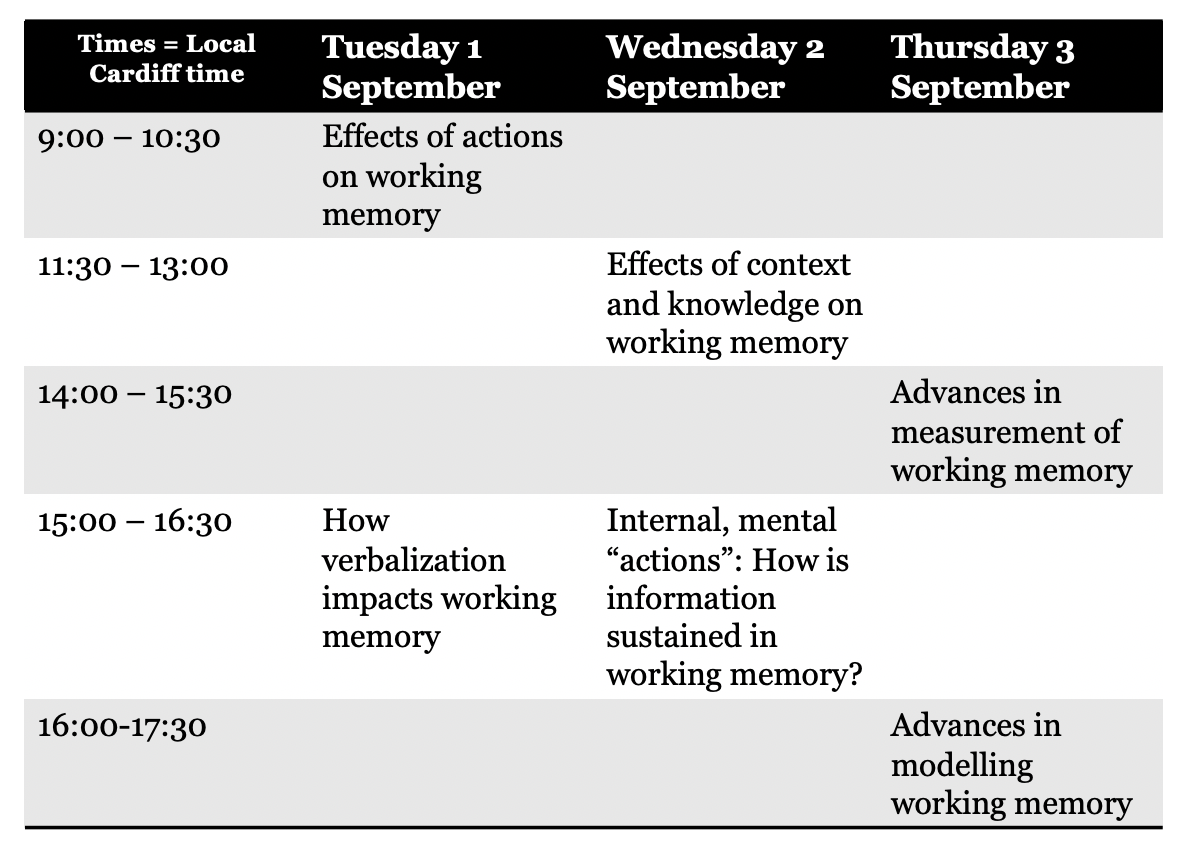
\includegraphics{ewomsSchedule.png}

\hypertarget{effects-of-actions-on-working-memory}{%
\chapter{Effects of actions on working memory}\label{effects-of-actions-on-working-memory}}

Actions may be considered extensions of memory, affording strategies for preserving information beyond what the capacity of working memory might typically allow. While study of speech-based sensory-motor phenomena is quite advanced, understanding how spatial and haptic sensory and motor functions influence memory remains under-explored. Talks in this session investigate non-speech sensory and motor influence on working memory, including motion, spatial awareness, and rhythmic pattern.

\hypertarget{schedule}{%
\section{Schedule}\label{schedule}}

This discussion session will take place 1 September from 9:00 - 10:30 (UK) / 10:00 - 11:30 (Switzerland/France) / 17:00 - 18:30 (Japan)

\hypertarget{abstracts}{%
\section{Abstracts}\label{abstracts}}

Recorded talks will be available from 14 August 2020.

\hypertarget{the-hebb-repetition-effect-in-reproduction-of-nonverbal-rhythms}{%
\subsection{The Hebb repetition effect in reproduction of nonverbal rhythms}\label{the-hebb-repetition-effect-in-reproduction-of-nonverbal-rhythms}}

\emph{Yoshiyuki Ueda (Kyoto University) \& Satoru Saito}

\emph{Email: \href{mailto:ueda.yoshiyuki.3e@kyoto-u.ac.jp}{\nolinkurl{ueda.yoshiyuki.3e@kyoto-u.ac.jp}}}

The Hebb repetition effect is a phenomenon that repeated presentation of the same sequence of memory items facilitate immediate serial recall performance of the sequence. This effect, which is predominantly tested in verbal domain, is assumed to exhibit the contributions of long-term knowledge to working memory. One of the notable characteristics of this effect is its strong dependence on presentation timing, as reflected in the decreased effect, which was observed when the temporal structures varied in each presentation of the repeated sequence. This suggests that the temporal structures are also learnt over repetition and might contribute to the Hebb repetition effect. The present study directly tested this assumption and investigated what mechanisms underlie it. In a series of immediate recall experiments, participants were presented multiple beep tones with rhythms and asked to reproduce it manually. In each experiment, one rhythm (the Hebb tone sequence) was frequently presented than others (the filler sequence). In Experiment 1, we confirmed the Hebb repetition effect in reproduction of nonverbal rhythms. In Experiment 2, participants were asked to engage in articulatory suppression during encoding the rhythm. The results showed no Hebb repetition effect under this situation, suggesting that either dual task demand or disruption of articulatory mechanisms might interfere with learning of temporal structures. In Experiment 3, participants were asked to perform either a visuospatial drawing task or articulatory suppression during the encoding. The results showed that the Hebb repetition effect for nonverbal rhythms was observed only for participants who performed the drawing task, indicating that the disappearance of the Hebb repetition effect in Experiment 2 was not due to the presence of dual-task demand. The findings reported here suggest that the temporal structure can be learnt over repetition through articulation related mechanisms.

\hypertarget{translating-words-into-actions-in-working-memory-a-role-for-spatial-motoric-coding-in-the-enacted-recall-advantage}{%
\subsection{Translating words into actions in working memory: a role for spatial-motoric coding in the enacted recall advantage}\label{translating-words-into-actions-in-working-memory-a-role-for-spatial-motoric-coding-in-the-enacted-recall-advantage}}

\emph{Richard Allen (University of Leeds), Guangzheng Li, Alan Baddeley, \& Graham Hitch}

\emph{Email: \href{mailto:r.allen@leeds.ac.uk}{\nolinkurl{r.allen@leeds.ac.uk}}}

The phonological loop component of working memory has benefited extensively from its application to understanding tasks of practical relevance. This is rather less so for the visuo-spatial sketchpad component although an exception is the recent range of studies concerned with the capacity to follow and enact spoken instructions in which enactment by the participant at recall has consistently been shown to produce enhanced performance. This is generally interpreted as reflecting a generated spatial-motoric plan, though the detailed characteristics of such a plan remain to be explored. We describe five experiments investigating this, comparing verbal and enacted recall of a series of actions under different concurrent task conditions involving repetitive actions that involve either fine motor (finger-based) or gross motor (arm-based) movement. A general advantage from enacted recall was observed across experiments, together with a tendency for concurrent action suppression to impair recall. The enacted recall advantage was reduced or abolished under certain concurrent action conditions, depending on factors such as complexity, familiarity, and gross vs.~fine motor movement. We conclude that our results are consistent with the view that spatial motoric plans are constructed in working memory for anticipated action.

\hypertarget{visuospatial-bootstrapping-spatialization-facilitates-verbal-memory-in-a-range-of-learning-and-memory-tasks}{%
\subsection{Visuospatial Bootstrapping: Spatialization facilitates verbal memory in a range of learning and memory tasks}\label{visuospatial-bootstrapping-spatialization-facilitates-verbal-memory-in-a-range-of-learning-and-memory-tasks}}

\emph{Stephen Darling (Queen Margaret University)}

\emph{Email: \href{mailto:sdarling@qmu.ac.uk}{\nolinkurl{sdarling@qmu.ac.uk}}}

There is growing evidence that spatial information that is available within visually presented materials can facilitate performance in verbal tasks. A frequently replicated finding demonstrates that immediate verbal serial recall is facilitated if the to-be-remembered items are presented in the familiar 2-dimensional PIN keypad. In this presentation I will summarise the key aspects of this literature, expanding from what is already known about immediate serial recall to research on long term sequence learning. I will then introduce a couple of recent studies. The first showed that bootstrapping-like responses occur in serial recall for non-numeric materials. The second showed that bootstrapping responses also occurred during `running span' tasks. Running span tasks are those where a participant is asked to remember the last items in a sequence, but is unaware of the sequence length, and so must keep the responses continually updated. Spatialized displays facilitated running span task recall. Additionally, the size of this benefit did not seem to be contingent on the speed of presentation. Overall, these findings tend to suggest that spatialization can enhance verbal memory when appropriate displays are used. This enhancement can occur in a range of different learning and memory tasks and operates relatively quickly and hence probably automatically.

\hypertarget{bootstrapping-the-visuospatial-bootstrapping-effect-and-testing-its-spatialisation}{%
\subsection{Bootstrapping the visuospatial bootstrapping effect (and testing its spatialisation)}\label{bootstrapping-the-visuospatial-bootstrapping-effect-and-testing-its-spatialisation}}

\emph{Alessandro Guida (Universitè Rennes)}

\emph{Email: \href{mailto:alessandro.guida.psychology@gmail.com}{\nolinkurl{alessandro.guida.psychology@gmail.com}}}

A decade ago, Darling and Havelka (2010) observed that when sequences of digits are visually presented within a numerical keypad on the screen (like those on phones), memory span increases. They called this phenomenon visuospatial bootstrapping (VB) to reflect the support of verbal memory by visuospatial memory. I will present two experiments that further investigate the power of VB and its consequence. The aim of the first experiment was to answer the following question: can the VB effect still emerge without actually presenting a keypad on the screen? For this purpose, a three-phase experiment was designed. During the first phase, the performances of two groups of participants in an immediate serial recall task were compared: the first group saw sequences of one-digit numbers displayed on a screen within a keypad (the keypad group) whereas the second group heard the (same) sequences (the auditive group). After this first phase, participants from both groups underwent an 18 minutes training phase in order to learn how to visualize in their mind's eye a numerical keypad and use it to encode sequences. Finally, in the third phase, participants were tested again in an immediate serial recall task similarly to phase one. Results showed that the VB effect can obtained without displaying a numerical keypad. The second experiment also involved a keypad group and an auditive group and was designed to investigate if the spatial representation of both groups were comparable. For this purpose, we adapted a paradigm from the study of the SPoARC effect (Spatial Positional Association Response Codes), which enables to test for a left-to-right or a right-to-left spatialization (or an absence of horizontal spatialization). Results showed that for both groups the spatial representation followed a left-to-right direction, compatible with the idea that participants associated the keys ``1'', ``4'', and ``7'' to left, ``2'', ``5'', and ``8'' to middle and ``3'', ``6'', and ``9'' to right.

\hypertarget{the-role-of-verbal-working-memory-in-gesturespeech-integration-the-need-of-taking-individual-differences-into-account}{%
\subsection{The role of verbal working memory in gesture/speech integration: The need of taking individual differences into account}\label{the-role-of-verbal-working-memory-in-gesturespeech-integration-the-need-of-taking-individual-differences-into-account}}

\emph{Kendra Kandana Arachchige (University of Mons), Henning Holle, Mandy Rossignol, Isabelle Simoes Loureiro, \& Laurent Lefebvre}

\emph{Email: \href{mailto:kendra.kandanaarachchige@umons.ac.be}{\nolinkurl{kendra.kandanaarachchige@umons.ac.be}}}

Iconic gestures (IG) are characterized by a formal relationship between the gesture and the speech it accompanies. It is now known that presenting semantically congruent (SC) IG (i.e.~that match the spoken utterance) compared to semantically incongruent (SI) ones improves comprehension. Since they occur concurrently to speech and are subject to on-line processing, Wu and Coulson (2014) suggested that verbal working memory (vWM) may play a role in gesture/speech integration (GSI). In a first study, participants were asked to complete a gender classification task (GCT), embedded in a vWM task where they were asked to remember words. Participants were presented with one or four words to remember (vWM task). The GCT consisted of videos of a gesture enacted by a man or a woman accompanied by a SC or SI audio from a man or woman's voice. Participants were asked to discriminate, as fast as possible, the gender of the voice. They then saw a list of words and had to click on the ones previously seen. This study failed to demonstrate an involvement of the vWM on GSI. We suggest that this may be due to not taking individual differences (ID) in vWM into account. We hence conducted a second study where we individualized the vWM task. We expect a main effect of SC shown by reduced reaction times for the SC condition compared to SI, and an interaction between vWM load and SC. 27 healthy French-speaking participants (6 men; Mage = 22.85; SD=0,79) completed the Digit Span Task, determining the span for the vWM. In the vWM, participants were here presented with one (low) or several (high load, matching their span) words. The GCT remained unchanged. A 3-way repeated-measures ANOVA (load(2)x semantics(2)xgender(2)) yielded significant main effect for semantics (F1,26 = 4,26; p = 0.04) with a faster processing of SC pairs, and an interaction effect load x semantic (F1,26 = 4,45; p = 0.04). These results suggest that vWM is indeed involved in GSI, but only when ID are taken into account.

\hypertarget{working-memory-at-play-two-studies-with-volleyball-players}{%
\subsection{Working memory at play: Two studies with volleyball players}\label{working-memory-at-play-two-studies-with-volleyball-players}}

\emph{Elisa Bisagno (University of Modena and Reggio Emilia), Sergio Morra, \& Francesca Vitali}

\emph{Email: \href{mailto:elisa.bisagno@unimore.it}{\nolinkurl{elisa.bisagno@unimore.it}}}

M capacity (Pascual-Leone, 1987; Pascual-Leone \& Goodman, 1979) has been found predictive of the performance in many perceptual, linguistic and reasoning tasks. However, it has been less studied ``in action'', for example, in the sport domain. We aimed at testing the role of M capacity in motor learning (Study 1) and sport performance (Study 2) in samples of youth volleyball players. Study 1 (Bisagno \& Morra, 2018): 105 youth female volleyball players (5-17 years old and a group of ``experts'', i.e.~adults with at least 10 years of volleyball experience) were engaged in WM tests and volleyball attack tasks of increasing difficulty, modelled via task analysis and scored in terms of ``correct execution'' and ``precision''. We also considered each athlete's experience (years of practice). The best predictor of the correct execution was the WM capacity, while experience was the only significant predictor of the precision. Also, a prediction analysis of cross-classification confirmed that M capacity sets a limit in learning certain attack gestures. Examples of our task analysis will be presented. Study 2 (under review): 114 youth female volleyball players (11-18 years old) were engaged in WM capacity and Executive Functions (updating, inhibition and shifting) tests. They also completed self-report measures with respect to their attentional style and precompetitive emotions. For each volleyball player, at least three competitions were recorded and scored by two expert observers. An individual performance index based on every gesture performed during the games, and controlled for the team performance, was computed. An M capacity-updating factor resulted as the main predictor of the volleyball players' performance, together with high-arousal ``unpleasant'' emotions. A moderation of emotional correlates on the relation between WM and performance was found. Taken together, these studies underline the role of capacity in predicting both motor learning and performance in volleyball.

\hypertarget{does-sensorimotor-arousal-influence-memory-functioning-a-test-of-embodied-view-of-memory-using-short-term-immobilization}{%
\subsection{Does sensorimotor arousal influence memory functioning? A test of embodied view of memory using short term immobilization}\label{does-sensorimotor-arousal-influence-memory-functioning-a-test-of-embodied-view-of-memory-using-short-term-immobilization}}

\emph{Jeremy Villatte (Universitè Poitiers), Laurence Taconnat, \& Lucette Toussaint}

\emph{Email: \href{mailto:jeremy.villatte@univ-poitiers.fr}{\nolinkurl{jeremy.villatte@univ-poitiers.fr}}}

In line with embodied views of cognition, growing evidence suggests that memory functioning is based on sensorimotor systems. Hence, different models (Versace et al., 2014; Briglia et al., 2018) assume that memory encoding rely on integration of sensorimotor information while retrieval is based on its reactivation. In the present study, we hypothesized that some memories are more strongly related to specific sensorial or motor systems that are crucial for their integration and reactivation. Example of this somatotopic-related memories could be observed using manipulable objects as stimuli. Thus, hand-related information is likely to play a more central role in memory of manipulable objects than information from other sensorimotor systems. In order to assess the specific contribution of manual sensorimotor system to memory of manipulable objects, we used a short term upper limb immobilization design. Twenty-four hours before the beginning of the experiment, a rigid splint was fixed on the dominant (right) hand of the participants assigned to the experimental group. The splint immobilized their hand, wrist and fingers. An immobilization vest restrained the move of their right arm to ensure they keep their hand at rest. Previous studies have shown that decreased arousal induced by immobilization elicit quick updating of manual sensorimotor representations (Meugnot \& Toussaint, 2015). Once twenty-four hours of immobilization elapsed, participants undergo a manipulable and non-manipulable objects pictures recognition task. We expected delayed response time for immobilized participants, in particular for correct recognitions (hits) of manipulable object. However, contrary to our prediction, hits for manipulable objects were faster for immobilized than for control group F (1,44) = 9,66, p\textless{}.01. We suggest that this surprising result is due to adaptive processes. Thus, immobilization could reduce amount of available information in memory, leading to quicker processing.

\hypertarget{visuo-spatial-working-memory-in-body-awareness-does-recalling-locations-helps-perceive-its-own-body}{%
\subsection{Visuo-spatial working-memory In body-awareness: does recalling locations helps perceive its own body?}\label{visuo-spatial-working-memory-in-body-awareness-does-recalling-locations-helps-perceive-its-own-body}}

\emph{Sara Salgues (Universitè Lyon), Gaën Plancher, \& George A. Michael}

\emph{Email: \href{mailto:Sara.salgues@univ-lyon2.fr}{\nolinkurl{Sara.salgues@univ-lyon2.fr}}}

Body-awareness requires maintaining body representations in focus. The perception of spontaneous sensations (SPS) in the absence of tactile stimulation of the skin would contribute to body-awareness. Vision and attention are predominant factors of body-awareness and of SPS perception, and contribute to the maintenance of representations in working memory. Lesions in the parietal lobe were found to impair the body-representation maintenance without visual focus, causing one to lose awareness of its body-parts within seconds. Given that spatial-vision and spatial-attention play an important role in SPS perception, it was hypothesized that visuo-spatial working memory (VSWM) would contribute to body-awareness, and thus modulate the perception of SPS. Computed VSWM tasks, in the form of a Brown-Peterson and a complex span tasks, and a standard task of SPS, investigating the perception of sensations perceived in the absence of any tactile stimulation on the hands, were proposed to participants. The effect of decay, interference and cognitive load on recall performances were extracted from the VSWM tasks. Correlational analyses were carried out between these values and SPS. This study found that slow decay, and low rates of forgetting due to cognitive load were mainly associated with higher frequency of SPS over the hand. Opposite patterns were observed for the interference: individuals with low rate of forgetting perceived more SPS on less sensitive area, and conversely. In conclusion, greater ability in working memory would contribute to a better perception of SPS, either through an increment of their frequency on the hand, or through a better sensitivity to SPS on less sensitive area of the hand. On previous studies, the perception of SPS on less sensitive area of the hand was associated to interoceptive abilities, also strongly linked to body-awareness. These findings allow us to discuss the involvement of VSWM in body-awareness.

\hypertarget{how-verbalization-impacts-working-memory}{%
\chapter{How verbalization impacts working memory}\label{how-verbalization-impacts-working-memory}}

How does verbalization impact memory for information, whether for words, images, or sounds? What does our understanding about interactions between verbalization and working memory performance suggest about the structure of a working memory system?

\hypertarget{schedule-1}{%
\section{Schedule}\label{schedule-1}}

This discussion session will take place 1 September from 15:00 - 16:30 (UK) / 16:00 - 17:30 (Switzerland/France) / 9:00 - 10:30 (USA - Central Time Zone)

\hypertarget{abstracts-1}{%
\section{Abstracts}\label{abstracts-1}}

Recorded talks will be available from 14 August 2020.

\hypertarget{when-does-spontaneous-verbal-rehearsal-emerge-in-children-and-how-does-it-effect-memory-recall-a-multi-lab-replication-of-flavell-beach-and-chinsky-1966}{%
\subsection{When does spontaneous verbal rehearsal emerge in children, and how does it effect memory recall? A multi-lab replication of Flavell, Beach and Chinsky (1966)}\label{when-does-spontaneous-verbal-rehearsal-emerge-in-children-and-how-does-it-effect-memory-recall-a-multi-lab-replication-of-flavell-beach-and-chinsky-1966}}

\emph{Candice C. Morey (Cardiff University), Emily M. Elliott, Angela AuBuchon, et al.}

\emph{Email: \href{mailto:moreyc@cardiff.ac.uk}{\nolinkurl{moreyc@cardiff.ac.uk}}}

\emph{Twitter: @CandiceMorey}

Work by Flavell, Beach, and Chinsky (1966) indicated a change in the spontaneous production of overt verbalization behaviors when comparing young children (age 5-6) to older children (age 10). Despite the critical role that this evidence of a change in verbalization behaviors plays in modern theories of cognitive development and working memory, there has only been one other published near-replication of this work (Keeney, Cannizzo, \& Flavell, 1967). This Registered Replication Report relied upon 17 labs who contributed their results to a larger and more comprehensive sample of children (N=980), with roughly equal numbers of 5-, 6-, 7-, and 10-year-olds. We assessed memory performance and the presence or absence of verbalization behaviors of young children across this age range, and determined that the original pattern of findings was largely upheld. We observed a clear increase in verbalization between 5- and 7-year-olds; however, the further increase between 7- and 10-year-olds the Flavell et al.~originally reported was much less clear. Verbalization was also more prevalent in the young children in our sample than it was in Flavell et al.'s sample, which seems inconsistent with the proposition that verbal rehearsal strategies are unavailable to children under 7. With our large sample, we were able to extend Flavell et al.'s findings with respect to the benefit of verbalization for recall. Children who verbalized, whatever their age, recalled longer sequences than children who did not. The implications for theories of working memory development arising from these findings will be discussed.

\hypertarget{how-do-verbal-labels-influence-childrens-visual-working-memory}{%
\subsection{How do verbal labels influence children's visual working memory?}\label{how-do-verbal-labels-influence-childrens-visual-working-memory}}

\emph{Clara Overkott (University of Zurich) \& Candice C. Morey}

\emph{Email: \href{mailto:c.overkott@psychologie.uzh.ch}{\nolinkurl{c.overkott@psychologie.uzh.ch}}}

Storage of information in visual working memory (WM) is highly constrained and only a limited amount of representations can be maintained vividly in mind. Verbal labeling can be used to improve visual WM. Research with young adults showed that labeling increases both the quantity and quality of the visual information retained in mind, and that adults tend to spontaneously use this strategy. So far, it is unclear whether children can and do use this strategy to improve their visual WM. In this study we aimed to assess developmental changes in verbal labeling effects on the storage of continuous (i.e., fine-grained) and categorical (more prototypical) color information, manipulating whether labeling was spontaneous or experimenter-instructed. Children (5-7 and 8-11 years) and young adults (18-35 years) did a delayed estimation task in which they memorized colored candies varying on a continuous scale. During memorization, they were prompted to remain silent, label the colors, or to say irrelevant syllabi (``bababa'') thereby discouraging verbal labeling. At test, the color of the candies was reproduced on a color wheel. Results showed that children of both age groups were able to spontaneously use verbal labels and engage in experimenter-instructed labeling. Across all age groups, experimenter-instructed labeling showed the highest labeling benefit. There was a developmental labeling benefit trend for both spontaneous and experimenter-induced labeling. Mixture modeling on the format (categorical or continuous) in which the colors were stored, and their precision showed that labeling increased both categorical and continuous storage as well as in precision for children over 7-years-old and under 7-years-old, as well as adults. This suggests that experimenter-instructed and spontaneous labeling benefits quantity and quality of visual information similarly across development.

\hypertarget{the-role-of-working-memory-maintenance-mechanisms-in-false-recall}{%
\subsection{The role of working memory maintenance mechanisms in false recall}\label{the-role-of-working-memory-maintenance-mechanisms-in-false-recall}}

\emph{Marléne Abadie (Aix Marseille University), Amelie Troubat, Christelle Guette, Valérie Camos}

\emph{Email: \href{mailto:marlene.abadie@univ-amu.fr}{\nolinkurl{marlene.abadie@univ-amu.fr}}}

Recent research revealed that working memory (WM) maintenance plays a crucial role in the occurrence of false recognition of semantically related lures (Abadie \& Camos, 2018). The present study explores the role of WM maintenance mechanisms, more specifically articulatory rehearsal and attentional refreshing, in false recall of semantic associates. In a Brown-Peterson paradigm, participants maintained lists of four semantically related words while performing a concurrent task. The attentional demand of the concurrent task and the presence of a concurrent articulation during the task were varied orthogonally to manipulate the availability of refreshing and rehearsal, respectively. Then, participants recalled the words immediately after the retention interval and in a delayed task occurring after each block of 10 trials. Results of two experiments provided decisive evidence that preventing the use of rehearsal or of refreshing reduces immediate correct recall. Interestingly, it also specifically increases immediate false recall of unpresented semantic associates with a stronger impact of articulatory suppression. Consistently in the two experiments, there was evidence against an effect of articulatory rehearsal on delayed recall performance. Refreshing also did not affect delayed recall performance in Exp.1. By contrast, in Exp. 2, in which participants were forced to recall the 40 words, i.e., the same number of words as words presented, there was strong evidence that preventing refreshing increased delayed correct recall and had no effect on false recall. These findings support the idea that rehearsal prevents the occurrence of short-term false memories but has no effect in the longer term. Refreshing would also reduce semantic distortions in the short-term, but the results are less clear as to its potential longer-term impact.

\hypertarget{false-memories-in-childrens-working-memory}{%
\subsection{False memories in children's working memory}\label{false-memories-in-childrens-working-memory}}

\emph{Rousselle Manon (Aix Marseille University), M. Abadie, V. Camos, \& A. Blaye}

\emph{Email: \href{mailto:manon.rousselle-jacquier@univ-amu.fr}{\nolinkurl{manon.rousselle-jacquier@univ-amu.fr}}}

Studies indicate that a memory can be distorted after only a few seconds (Atkins \& Reuter-Lorenz, 2008). Working memory (WM) maintenance mechanisms seem to determine the occurrence of false memory at short-term (Abadie \& Camos, 2018). In this study, we examined this phenomenon by comparing the occurrence of false memories in 4 y.o children, who do not yet use any WM maintenance mechanisms, and 8 y.o children, who spontaneously use maintenance strategies (Oftinger \& Camos, 2016). Children performed a Brown-Peterson task in which they had to memorize semantically related items lists. Then they did an 8-second concurrent task. The difficulty of this task was varied to manipulate maintenance of memory items through WM. Afterwards, children performed a recognition task composed of target items, and of distractors semantically related and unrelated to the memory items. Results provided substantial evidence against an effect of age on correct recognition of targets and indicated that 4 y.o. falsely recognized related distractors as targets more often than 8 y.o. Unfortunately, our manipulation of WM maintenance mechanisms was probably not strong enough to affect children recognition performance. Data were also analyzed with the conjoint recognition model of the Fuzzy-trace theory (Brainerd et al., 1999) to estimate the contribution of gist and verbatim memory to recognition performance. Interestingly, 8 y.o. retrieved more gist and verbatim memory than 4 y.o. These findings suggest that both gist and verbatim memory increase with age which specifically reduce false recognition in working memory.

\hypertarget{working-memory-and-language-actions-load-effects-on-quality-control-in-preschool-childrens-production-of-novel-syntax}{%
\subsection{Working memory and language actions: Load effects on quality control in preschool children's production of novel syntax}\label{working-memory-and-language-actions-load-effects-on-quality-control-in-preschool-childrens-production-of-novel-syntax}}

\emph{Eryn Adams (University of Missouri) \& Nelson Cowan}

\emph{Email: \href{mailto:erynadams@mizzou.edu}{\nolinkurl{erynadams@mizzou.edu}}}

Working memory is widely accepted as a necessary resource for a wide variety of cognitive abilities. Developmental work has shown that as working memory capacities increase, so too does the ability to successfully perform other cognitive tasks, including language comprehension and production. The present work demonstrates effects of working memory availability on language production. Whereas most of the previous research linking working memory to language development has been correlational, we experimentally varied the working memory load during concurrent language production in children 4-5 years old. Participants (N=36) were asked to repeat verbatim the previously heard, passive-voice descriptions of images displaying transitive-verb actions. These responses were performed while children sometimes retained a spatial-visual or verbal working memory load to be recalled after sentence production. Responses were coded for either maintaining the relatively unfamiliar passive voice of a previously heard description of the picture, or changing the syntax to a more familiar, active voice. Surprisingly, children were more likely to use the active voice when there was no concurrent working memory load. Under a load, children more often used the passive voice, as they were instructed to do, but produced more errors while doing so (including some nonsensical renditions such as the girl was watered by the flower). We propose that working memory, when available, is used to impose a quality-control process whereby the semantic fidelity of the response to the stimulus picture is preserved, here at the expense of disregarding the experimental instruction to reproduce the passive voice.

\hypertarget{short-term-memory-for-music-the-role-of-the-vocal-motor-system}{%
\subsection{Short-term memory for music: the role of the vocal motor system?}\label{short-term-memory-for-music-the-role-of-the-vocal-motor-system}}

\emph{Simon Gorin (University of Geneva) \& Emma Greenspan}

\emph{Email: \href{mailto:gorinsimon@gmail.com}{\nolinkurl{gorinsimon@gmail.com}}}

Whether people engage in covert rehearsal to maintain musical information in short-term memory (STM) is unclear. In this study, we tested the hypothesis that the maintenance of pitch information in STM is supported by the vocal motor system. More precisely, we tested the idea that the rehearsal of pitch information relies on the translation of an auditory target into the motor codes required to reproduce that target. The same sensorimotor translation mechanism is assumed to operate in pitch imitation, and studies on singing abilities showed that the closest from participants' voice is the to-be-imitated the target, the most accurate is their imitation. Consequently, if the vocal motor system supports the maintenance of pitch information in a recognition task for pairs of melodies, we should observe better recognition performance with material sounding with the timbre of a synthetic voice than a piano (Experiment 1) and for melodies with the timbre of a real voice than a synthetic voice (Experiment 2). Also, it is expected that the effect of the type of timbre should disappear under articulatory suppression but not under manual tapping as only the former recruits the vocal motor system. In Experiment 1, we observed no effect of the type of timbre. In Experiment 2, the participants showed an advantage such that recognition was better for melodies with a real voice compared to melodies with a synthetic voice. However, as expected, this advantage disappeared with articulatory suppression. Our results suggest the existence of a link between the vocal motor system and the mechanism involved in pitch maintenance in STM.

\hypertarget{effects-of-context-and-knowledge-on-working-memory}{%
\chapter{Effects of context and knowledge on working memory}\label{effects-of-context-and-knowledge-on-working-memory}}

What are the mechanisms underlying the influence of long-term memory knowledge (e.g., semantic or feature similarity, chunking) on working memory? Talks in this session address topics such as how these LTM influences are at play at the level of encoding, relative to at retrieval, and whether we can determine the direction of LTM-WM relationships (e.g., language learning and verbal working memory)? Other talks in this session consider factors such as attention, refreshing and emotion in relation to the effects of context and knowledge on working memory.

\hypertarget{schedule-2}{%
\section{Schedule}\label{schedule-2}}

This discussion session will take place 2 September from 11:30 - 13:00 (UK) / 12:30 - 14:00 (Switzerland/France)

\hypertarget{abstracts-2}{%
\section{Abstracts}\label{abstracts-2}}

Recorded talks will be available from 14 August 2020.

\hypertarget{syntax-morphosyntax-and-serial-recall-how-language-supports-short-term-memory-for-order}{%
\subsection{Syntax, morphosyntax, and serial recall: How language supports short-term memory for order}\label{syntax-morphosyntax-and-serial-recall-how-language-supports-short-term-memory-for-order}}

\emph{Judith Schweppe (University of Erfurt), Friederike Schuette \& Marie Hellfritsch}

\emph{Email: \href{mailto:judith.schweppe@uni-erfurt.de}{\nolinkurl{judith.schweppe@uni-erfurt.de}}}

In the classic view of verbal short-term memory, immediate recall of verbal sequences is achieved by maintaining phonological representations via articulatory rehearsal, while the influence of other linguistic information is negligible. According to language-based accounts, short-term retention of verbal material is inherently bound to language production and comprehension, thus also influenced by semantic or syntactic factors. In line with this, serial recall of word lists is better when they are presented in a canonical word order for English rather than in a non-canonical order, e.g., when adjectives precede nouns rather than vice versa, even when they are semantically unrelated (Perham, Marsh, \& Jones, 2009, QJEP). However, in many languages, grammaticality is not exclusively determined by word order. In German, for instance, an adjective-noun sequence is grammatical only if the adjective is inflected in congruence with the noun's person, number, and grammatical gender. Therefore, we investigated whether similar effects of syntactic word order occur in serial recall of lists in German. In a modified replication of Perham et al.'s study, we presented lists of 3 pairs of adjectives and nouns. We manipulated ordering (adjective-noun vs noun-adjective) and morphosyntactic congruence between nouns and adjectives within pairs (adjectives inflected vs uninflected). Recall performance benefited from an adjective-noun order only when adjectives were inflected. However, recall for the lists with uninflected adjectives was as good as in the most grammatical condition. As uninflected adjectives are shorter, this may be due to a confound with word length, an assumption we aim to test in a follow-up experiment. Nonetheless, the current findings are in line with language-based models and indicate that, in a language that determines grammaticality in an interplay of syntactic and morphosyntactic factors, word order alone is not sufficient to improve verbal short-term memory.

\hypertarget{short-term-memory-digit-span-scores-as-a-consequence-not-cause-of-language-learning}{%
\subsection{Short-term memory (digit) span scores as a consequence not cause of language learning}\label{short-term-memory-digit-span-scores-as-a-consequence-not-cause-of-language-learning}}

\emph{Gary Jones (Nottingham Trent University), Lucy V. Justice, Francesco Cabiddu, Bethany J. Lee, Lai-Sang Iao, Natalie Harrison, Bill Macken}

\emph{Email: \href{mailto:gary.jones@ntu.ac.uk}{\nolinkurl{gary.jones@ntu.ac.uk}}}

Such is the consistency by which performance on measures of short-term memory (STM) increase with age that developmental increases in STM capacity are largely accepted as fact. Maturational capacity increases show strong links to higher order cognitive function - particularly language learning - that place STM at the heart of any explanation of such learning. However, our analysis of a robust but almost ignored finding - that span for digit sequences (the traditional measure of STM) increases at a far greater rate than span for other verbal material - fundamentally undermines the assumption that increased performance in STM tasks is underpinned by developmental increases in capacity. We show that this digit superiority with age effect is explained by the relatively greater linguistic exposure to random sequences of digits versus other stimuli such as words. A simple associative learning process that learns incrementally from exposure to language accounts for the effect, without any need to invoke an STM mechanism, much less one that increases in capacity with age. By extension, using corpus data directed at 2-3 year old children, 4-6 year old children, and adults, we show that age-related performance increases with other types of verbal material are equally driven by the same basic associative learning process operating on the expanding exposure to language experienced by the child. Our results question the idea that tests such as digit span are measuring a dedicated system for the temporary maintenance and manipulation of verbal material, and as such have implications for our understanding of those aspects of child development that are usually accounted for with respect to the operation of such a system. In particular, our results suggest that increases in STM performance do not play a causal role in language learning, but rather language learning itself is what causes increased performance in verbal STM tasks.

\hypertarget{working-memory-and-vocabulary-breadth-and-depth-how-they-contribute-to-explain-reading-comprehension}{%
\subsection{Working memory and vocabulary breadth and depth: How they contribute to explain reading comprehension}\label{working-memory-and-vocabulary-breadth-and-depth-how-they-contribute-to-explain-reading-comprehension}}

\emph{Paola Palladino (University of Pavia) \& Caterina Artuso}

\emph{Email: \href{mailto:paola.palladino@unipv.it}{\nolinkurl{paola.palladino@unipv.it}}}

Vocabulary knowledge has been usually conceptualized and investigated as the number of words known (i.e., a measure of vocabulary breadth). However, research has shown the benefit of considering at least two dimensions of vocabulary knowledge: breadth and depth (e.g., Oakhill et al.,2015; Ouellette, 2006). In particular, these two dimensions have been related to reading comprehension showing contradictory results: for some researchers breadth has a stronger relation to comprehension that does depth (e.g., Tannenbaum, 2006), for some others breath predicts word encoding whereas depth predicts comprehension (Ouellette, 2006). The aim of the current study is to investigate how these two vocabulary dimensions account for variance in reading comprehension also considering the contribution of short-term and working memory, separately. Fifty children from third grade (mean age 8.4 years) were administered a series of tasks to assess their short-term memory, working memory, vocabulary depth (from the WISC IV) and breadth (taken from an Italian developmental neuropsychological assessment battery), and comprehension (assessed with an Italian standardized inferential comprehension task). Main finding indicated that working memory (but not short-term) explained vocabulary depth; vocabulary breadth was not accounted for by these memory measures. However, when both vocabulary breadth and depth, as well as memory measures, were entered to explain inferential reading comprehension, we found that WM lost its significance and vocabulary depth only accounted for reading comprehension. The study suggests the relevance to distinguish vocabulary breadth and depth in order to better capture the role of working memory in reading comprehension. It gives an original hint to sketch the mediational role of vocabulary depth from working memory to inferential reading comprehension.

\hypertarget{resource-reallocation-in-working-memory-through-semantic-chunks-computational-and-behavioural-evidence}{%
\subsection{Resource reallocation in working memory through semantic chunks: Computational and behavioural evidence}\label{resource-reallocation-in-working-memory-through-semantic-chunks-computational-and-behavioural-evidence}}

\emph{Benjamin Kowialiewski (Université Grenoble Alpes), Benoît Lemaire, \& Sophie Portrat}

\emph{Email: \href{mailto:bkowialiewski@uliege.be}{\nolinkurl{bkowialiewski@uliege.be}}}

\textbf{Introduction}: Many studies have shown that long-term memory knowledge, such as semantic knowledge, supports the short-term maintenance of verbal information in Working Memory (WM). For instance, it has been shown that to-be-remembered items related at the semantic level (e.g.~leaf, tree, branch) are better recalled as compared to unrelated items (e.g.~wall, sky, dog). However, the mechanisms underlying the influence of semantic knowledge in WM remain poorly understood. In this study, we took advantage of a convergent approach involving computational and behavioural methods to assess the possibility that semantic knowledge can be used in order to save WM resources that can be efficiently reallocated for maintenance purposes.

\textbf{Methods \& Results}: In an experiment requiring participants to perform immediate serial recall of lists composed of six memoranda (e.g.~leaf - tree - branch - wall - sky - dog), we observed that the presence of a semantic chunk (i.e.~leaf - tree - branch) enhanced recall performance for items that directly followed the semantic chunk (i.e.~wall - sky - dog), and this compared to a condition where all the items were semantically unrelated (e.g.~hammer - jacket - horn - wall - sky - dog). This phenomenon is successfully captured by a new computational architecture in which we integrated the activation occurring in the long-term memory linguistic system (Dell et al., 1997) within TBRS*, a decay-based WM model (Oberauer \& Lewandowsky, 2011).

\textbf{Conclusion}*: In this study, not only do we show for the first time that semantic knowledge can be used in order to save WM resources, but our simulations also demonstrate the potentialities offered by bridging the gap between WM and the activation in the long-term memory system.

\hypertarget{does-attentional-refreshing-modulate-the-associative-relatedness-effect-in-children-and-adults-working-memory}{%
\subsection{Does attentional refreshing modulate the associative relatedness effect in children and adults' working memory?}\label{does-attentional-refreshing-modulate-the-associative-relatedness-effect-in-children-and-adults-working-memory}}

\emph{Fiona Laura Rosselet-Jordan (University of Fribourg), Marléne Abadie, Stephanie Mariz Elsig, \& Valérie Camos}

\emph{Email: \href{mailto:fionalaura.rosselet-jordan@unifr.ch}{\nolinkurl{fionalaura.rosselet-jordan@unifr.ch}}}

Long-term memory (LTM) is known for affecting recall during working memory (WM) tasks. However, the way LTM intervenes in WM remains unknown. To test the predictions issued from different WM models (Barrouillet, Bernardin, \& Camos, 2004; Cowan, 1999; Rose, Buschsbaum, \& Craik, 2014), the involvement of semantic LTM representations in a complex span task was manipulated through variations of the associative relatedness of the memory items, while the attentional demand of the concurrent task was varied to manipulate refreshing opportunities. Children and young adults were also compared, because children should use refreshing and relatedness cues less efficiently than adults. Despite the impact of the three main factors on recall performance which was better for related than unrelated words, with the low rather than the high demanding concurrent task and for adults than children, there was no interaction between associative relatedness and attentional demand neither in children nor in adults. We replicated these results in a second experiment with a more demanding secondary task. Moreover, the impact of the three mentioned factors was also analyzed on recall latency. In accordance with recall performance, participants, especially adults, were faster at recalling related (vs.~unrelated) words, without any effect of the concurrent attentional demand on recall latency. The present findings suggest that the availability of attention does not modulate the effect of LTM on WM. We discuss how WM models can account for this finding and how LTM acts on WM functioning.

\hypertarget{no-detrimental-effect-of-semantic-similarity-on-order-memory-could-an-encoding-benefit-be-the-explanation}{%
\subsection{No detrimental effect of semantic similarity on order memory: Could an encoding benefit be the explanation?}\label{no-detrimental-effect-of-semantic-similarity-on-order-memory-could-an-encoding-benefit-be-the-explanation}}

\emph{Julia Krasnoff (University of Zurich), Eda Mizrak, \& Klaus Oberauer}

\emph{Email: \href{mailto:j.krasnoff@psychologie.uzh.ch}{\nolinkurl{j.krasnoff@psychologie.uzh.ch}}}

Similarity between items in a list can facilitate and impair working memory performance. For instance, phonological similarity enhances item but impairs order memory. This finding is explained by processes during retrieval where similar items serve as cues for each other, facilitating their retrieval but not necessarily in the right position. In two experiments using a serial-recall task with six-word lists we examined whether semantic similarity affects memory likewise. In experiment 1, semantic similarity was operationalized through 1) latent semantic analysis (LSA) or 2) categorical similarity. For both conditions, similarity improved item and, surprisingly, did not harm order memory. The effect was mainly driven by performance of the last three items, casting doubt on a solely retrieval-based explanation, which would predict similar effects for all items. In experiment 2, we tested whether there is an encoding benefit for semantically similar items that compensates the detrimental effect during retrieval. We considered the idea of an encoding resource (Popov \& Reder, 2020) that depletes with each encoded item and combined it with the idea that similar items consume fewer resource due to activation of a common category at encoding. This leads to the prediction that items preceded by semantically similar items are left with more encoding resource and hence are better recalled even if being semantically unrelated. To test this, we manipulated similarity between first and second part of lists. Participants studied six-word lists of 1) similar, 2) dissimilar, 3) three similar followed by three dissimilar, 4) three dissimilar followed by three similar words. As predicted, performance for the second part was better when preceded by similar as compared to dissimilar words. This suggests that semantic similarity between items facilitates their encoding, saving encoding resource for the following items, and counteracting any detrimental effect of similarity at retrieval.

\hypertarget{the-effects-of-spacing-in-incidental-chunk-learning}{%
\subsection{The effects of spacing in incidental chunk learning}\label{the-effects-of-spacing-in-incidental-chunk-learning}}

\emph{Krzysztof Piątkowski (SWPS University), Katarzyna Zawadzka \& Maciej Hanczakowski}

\emph{Email: \href{mailto:kpiatkowski1@swps.edu.pl}{\nolinkurl{kpiatkowski1@swps.edu.pl}}}

To date, working memory studies examining chunking have mostly used procedures of deliberate learning. However, pre-experimentally established chunks examined in the working memory literature, such as well-known acronyms (e.g.~FBI, CIA, IBM), are learned not intentionally, but rather acquired incidentally while performing tasks such as reading or problem solving. Here we examined how chunks are acquired and then utilized in a decision-making task requiring short-term memory maintenance. Using a variant of the task span paradigm (Logan, 2004), we repeatedly presented strings of letters, each denoting a binary decision to be made for visual stimuli. Performance in this task required short-term maintenance of strings in service of performing cognitive operations in a correct order. In the acquisition phase we manipulated whether repetitions of strings were massed or spaced. In the test phase, performance for strings from the acquisition phase was compared to performance for novel strings. In Experiment 1, both massed and spaced presentations improved performance when the same strings were re-used in the test phase, and to the same extent. In Experiment 2, memory load was introduced in the test phase in the form of to-be-remembered digits in order to assess whether newly created chunks free cognitive resources. Here again performance in the main task was equally facilitated for strings acquired in a massed and spaced fashion, but only chunks acquired in a spaced fashion improved performance in the secondary memory task.
Our results suggest that memory chunks can be acquired incidentally, both by spaced and massed repetitions, and these chunks support redintegration responsible for reconstructing order of operations denoted by a chunk. On the other hand, only spaced acquisition seems to support chunks that not only help to redintegrate information but also to compress it when performing a complex task, so that additional information can be maintained in working memory.

\hypertarget{working-memory-and-categorization-how-people-code-information-in-working-memory-when-items-share-features}{%
\subsection{Working memory and categorization: How people code information in working memory when items share features?}\label{working-memory-and-categorization-how-people-code-information-in-working-memory-when-items-share-features}}

\emph{Gaën Plancher (University of Lyon) \& Robert Goldstone}

\emph{Email: \href{mailto:gaen.plancher@univ-lyon2.fr}{\nolinkurl{gaen.plancher@univ-lyon2.fr}}}

A large literature suggests that the way we process information is influenced by the categories that we have learned. We examined whether when we try to uniquely encode items in working memory, the information encoded depends on the other stimuli being simultaneously learned. Participants were required to memorize unknown aliens, presented one at the time, for immediate recognition of their features. Some aliens, called twins, were organized into pairs that shared every feature (non-discriminative feature) except one (discriminative feature), while some other aliens, called hermits, did not share feature. We reasoned that if people develop unsupervised categories by creating a category for a pair of aliens, we should observe better feature identification performance for non-discriminative features compared to hermit features, but not compared to discriminative features. On the contrary, if distinguished feature draws attention, we should observe better performance when a discriminative rather than non-discriminative feature was probed. Our results showed that accuracy for non-discriminative features was equivalent to accuracy for discriminative features, but performance was greater for non-discriminative probes compared to hermit. Also, correlations in accuracy for parts in a twin were higher than correlations in accuracy for parts across twins. Finally, errors were greater for discriminative twin features than other kind of probes. This difference was accentuated by training, suggesting that features within the same cluster acquired equivalence over time. Overall, this suggests that when items share features, people code items in working memory by focusing on similarities between items, establishing clusters of items based in an unsupervised fashion not requiring feedback on cluster membership.

\hypertarget{impacts-of-anxiety-on-executive-and-perceptual-attention-in-visual-working-memory}{%
\subsection{Impacts of anxiety on executive and perceptual attention in visual working memory}\label{impacts-of-anxiety-on-executive-and-perceptual-attention-in-visual-working-memory}}

\emph{David Spalding (University of Strathclyde), Louise A. Brown Nicholls, \& Marc Obonsawin}

\emph{Email: \href{mailto:david.m.spalding@strath.ac.uk}{\nolinkurl{david.m.spalding@strath.ac.uk}}}

Trait anxiety is associated with deficits in attentional control, whereby top-down, directed executive control is diminished at the expense of bottom-up, perceptually driven attentional capture. Meanwhile, effective binding of features in visual working memory has been shown to rely on these processes, specifically when to-be-remembered objects are presented sequentially over time. Despite evidence for negative impacts of anxiety on visual working memory, there has been little study of the impacts of anxiety on binding specifically. Such studies would help to clarify the role of anxiety, and emotion more broadly, within multicomponent working memory models. Two studies will be presented that investigate the impact of trait anxiety on performance in a change detection, sequential binding task. Study 1 varied perceptual complexity, comparing memory for bindings (coloured shapes) to memory for individual features (blank shapes across varying array sizes (3 vs 4 items). Study 2 compared binding performance only. Participants performed either a concurrent task in which they count backwards from a two-digit number in threes - increasing executive demand - or repeat a two-digit number, a control condition engaging articulatory suppression. Outcomes will be measured in terms of performance effectiveness (proportion correct response accuracy) and efficiency (response times in trials in which a correct response was given). Results will indicate the extent to which trait anxiety impacts on visual feature binding in working memory, and the extent to which this is driven by specific anxiety symptoms (trait-cognitive or trait-somatic), task demand (memory for 3 or 4 items), attentional load (backwards counting or articulatory suppression), and/or memory type (binding or individual feature memory), as well as the potential interactions between these factors.

\hypertarget{internal-mental-actions-how-is-information-sustained-in-working-memory}{%
\chapter{Internal, mental ``actions'': How is information sustained in working memory?}\label{internal-mental-actions-how-is-information-sustained-in-working-memory}}

Talks in this session cover the nature of refreshing in WM and how refreshing supports maintenance. This includes investigation of the retro-cue effect and the mechanisms underlying it, as well as the relationship between retrospective attention and working memory. This session also covers the topic of how WM maintenance processes (e.g.~refreshing, binding) may change over the course of development/ageing.

\hypertarget{schedule-3}{%
\section{Schedule}\label{schedule-3}}

This discussion session will take place 2 September from 15:00 - 16:30 (UK) / 16:00 - 17:30 (Switzerland/France)

\hypertarget{abstracts-3}{%
\section{Abstracts}\label{abstracts-3}}

Recorded talks will be available from 14 August 2020.

\hypertarget{developmental-changes-in-retrospective-attention-influence-visual-working-memory-precision}{%
\subsection{Developmental changes in retrospective attention influence visual working memory precision}\label{developmental-changes-in-retrospective-attention-influence-visual-working-memory-precision}}

\emph{Gaia Scerif (University of Oxford) \& Andria Shimi}

\emph{Email: \href{mailto:gaia.scerif@psy.ox.ac.uk}{\nolinkurl{gaia.scerif@psy.ox.ac.uk}}}

Visual working memory (VWM) improves dramatically during childhood but what drives this improvement is not well understood. One influential account thus far has been a simple increase in storage capacity. However, recent findings have shown that differences in the ability to use attention retrospectively to enhance the maintenance of internal representations are also important for understanding developmental improvements in VWM. Yet, changes in this ability are not the sole contributor to developmental differences in VWM performance. Indeed, additional findings have indicated developmental changes in VWM precision. In this study, we aimed to examine whether the developing ability to orient attention retrospectively to internal representations influences VWM precision differentially for children than for adults. To do so, we employed a paradigm that combined the continuous-recall VWM task with the partial-cueing report task. Specifically, seven-year-olds and young adults were asked to reproduce the colour of a probe item in a colour-wheel. The initial memory array, which included the probe item, could be uncued or followed by a spatial cue (retrocue) that directed participants' attention to a location in the memory array. Results showed that attentional biases engendered by retro-cues facilitated fidelity (overall precision) compared to uncued, baseline performance, for both age groups, but to a smaller degree in 7-year-olds compared to adults. Importantly, investigation of modelling parameters suggested that children demonstrate lower representational fidelity of items in VWM and that spatial attentional cues improve overall precision by increasing the probability of target storage, maintenance and recall, and by reducing misbinding errors as well as random guessing. These results extend our knowledge on the relation between retrospective attention and VWM development.

\hypertarget{on-maintenance-of-continuous-representation}{%
\subsection{On maintenance of continuous representation}\label{on-maintenance-of-continuous-representation}}

\emph{M. Labaronne (Universitè Lyon), S. Harding, R. Shiffrin, \& G. Plancher}

\emph{Email: \href{mailto:maximilien.labaronne@univ-lyon2.fr}{\nolinkurl{maximilien.labaronne@univ-lyon2.fr}}}

Working memory performance for categorical items such as letters is a linear function of the cognitive load of a concurrent task, giving evidence that memory traces are maintained through attentional refreshing. The present study tested the effect of a concurrent load upon precision of memory for colors. Participants were asked to remember a series of three colors presented sequentially on a screen, each color was followed by three digits to be categorised. The cognitive load of the concurrent task was manipulated by varying the pace of digits presentation. At the end of the trial on a color wheel, participants were required to provide sequentially their best guess about the three colors they remembered, but also to provide a confident interval around their guesses. The same experiment was also conducted under articulatory suppression. Cognitive load affected the distance of the point estimate of color to the correct color, but not the width of the confidence interval, except for the third color. Articulatory suppression decreased memory performance and confidence and this effect did not interact with cognitive load. These findings suggested that continuous representation can be maintained through attentional refreshing.

\hypertarget{investigating-the-differences-between-the-types-of-bindings-underlying-working-memory}{%
\subsection{Investigating the differences between the types of bindings underlying working memory}\label{investigating-the-differences-between-the-types-of-bindings-underlying-working-memory}}

\emph{Maria Sanz Taberner (University of Essex) \& Vanessa Loaiza}

\emph{Email: \href{mailto:msma17029@essex.ac.uk}{\nolinkurl{msma17029@essex.ac.uk}}}

Binding, or mentally amalgamating different details of studied information,is an important factor underlying working memory (WM).We investigated the potential dissociation between different types of binding memory in an adaptive WM task (Bartsch et al., 2018), wherein participants studied three random letter pairs (e.g., L S, F‚Q, HX) each presented in different font colours (e.g., red, blue, green). Thereafter, participants were probed with one of the letters (e.g., F) from each pairing to recall its associated letter and font colours in two respective rows of three options: the correct target (e.g., Q, blue), a never-presented lure (e.g., Z, pink), and a lure from a different pair (e.g., S, red).The experiment comprised three blocks, each of them adjusting the presentation rate of subsequent trials based on the participants' colour accuracy, letter accuracy, and the combined accuracy of both details to achieve an approximate 67\% criterion in each block. We applied a hierarchical Bayesian multinomial processing tree (MPT) model to the observed frequencies of the three different types of responses to derive latent parameter estimates of intrinsic binding memory (i.e., remembering the font colour of the presented pair of letters), extrinsic binding memory (i.e., remembering the pairing between the letters),and joint binding memory (e.g., integrating the letters with their font colour). We found that the presentation rate was sensitive to the block adjustment, such that the letter block (M= 1.77, SD= 1.03) was faster than the colour block (M= 3.30, SD= 1.06), which in turn was faster than the combined block (M= 4.64, SD= 1.10). Interestingly, the block adjustment only impacted joint binding memory, with no credible differences between the blocks for intrinsic or extrinsic binding memory. These results suggest a dissociation of the different types of binding underlying WM.

\hypertarget{strategic-prioritisation-enhances-young-and-older-adults-visual-feature-binding-in-working-memory}{%
\subsection{Strategic prioritisation enhances young and older adults' visual feature binding in working memory}\label{strategic-prioritisation-enhances-young-and-older-adults-visual-feature-binding-in-working-memory}}

\emph{Louise A. Brown Nicholls (University of Strathclyde), Amy Atkinson, \& Richard J. Allen}

\emph{Email: \href{mailto:l.nicholls@strath.ac.uk}{\nolinkurl{l.nicholls@strath.ac.uk}}}

Young (18-33 yrs) and older (60-90 yrs) adults' ability to retain visual feature bindings in working memory was assessed, as was the extent to which memory could be enhanced using strategic prioritisation. The task involved sequentially presenting three coloured shapes, followed by a test probe in the form of an individual colour or shape, and participants were asked to recall the accompanying feature. Based on previous evidence, the earlier sequential objects are most vulnerable to forgetting, and in older adults this is especially so for the middle object. In Experiment 1, participants were instructed either to focus on all objects equally, or to prioritise a particular object in the array that was deemed more valuable (i.e.~more points would be awarded if that object was probed and recalled correctly). As older adults may not be as strategically flexible as young adults, they might differentially benefit from instructions to focus attention on certain objects, especially for the most vulnerable ones. As expected, young adults outperformed older adults overall. A general recency effect was also found, and the poorest performance was observed at the middle serial position. Additionally, both age groups were equally able to prioritise an object in visual working memory, with the largest effects observed at the most vulnerable middle position. Experiment 2 investigated the potential effect of increasing encoding time. This replicated the findings from Experiment 1, but further showed that, under these conditions, processing speed does not limit older adults' ability to benefit from strategic prioritisation.

\hypertarget{is-inhibition-in-working-memory-domain-general-a-study-of-age-related-decline-in-cross-domain-inhibitory-abilities}{%
\subsection{Is inhibition in working memory domain-general? A study of age-related decline in cross-domain inhibitory abilities}\label{is-inhibition-in-working-memory-domain-general-a-study-of-age-related-decline-in-cross-domain-inhibitory-abilities}}

\emph{Coline Grégoire (Universitè de Liège) \& Steve Majerus}

\emph{Email: \href{mailto:coline.gregoire@doct.uliege.be}{\nolinkurl{coline.gregoire@doct.uliege.be}}}

The unitary versus non-unitary nature of inhibitory control in working memory remains an open question: does inhibitory control deficit (i.e.~to inhibit irrelevant information) appearing during aging concern all domains (language or visual information, etc.) or are they more important in certain areas (language) than others (visual information)? This study examines the specificity of inhibitory control by investigating the age-related decline in inhibitory abilities across several domains (visual, phonological and semantic) in an immediate target-probe matching task. 129 young adults (20-40 years old) and 130 elderly adults (60-80 years old) where presented two target stimuli and two probe stimuli (visual symbols, words or nonwords); they had to select the probe stimulus that was the most similar to both target stimuli based on visual, semantic or phonological similarity. In the inhibition condition, the wrong probe stimulus was pre-activated via a prime stimulus briefly occurring before the presentation of the target stimuli and thus had to be inhibited for correct response selection; in the facilitation condition, the correct probe stimulus was preactivated. An interference score was calculated by subtracting performance between the two conditions, for each stimulus domain. We observed that interference effects were overall larger in the elderly adults as compared to the young adult group. At the same time, there was decisive Bayesian evidence for an interaction between age group and stimulus domain, with particularly increased interference effects in the elderly group for the semantic and visual conditions. These results suggest domain general inhibition impairment at least for semantic and visual conditions in healthy aging. Differences in task sensitivity may account for the lesser inhibition impairment in the phonological domain.

\hypertarget{working-memory-and-attention-a-computational-model-of-retro-cue-effects}{%
\subsection{Working memory and attention: A computational model of retro-cue effects}\label{working-memory-and-attention-a-computational-model-of-retro-cue-effects}}

\emph{Klaus Oberauer (University of Zurich)}

\emph{Email: \href{mailto:k.oberauer@psychologie.uzh.ch}{\nolinkurl{k.oberauer@psychologie.uzh.ch}}}

Directing attention to a subset of the contents of working memory improves the speed, and often the accuracy, of accessing the attended information. This can be demonstrated with the retro-cue paradigm (Souza \& Oberauer, 2016), in which an item in the memory set is cued as most likely to be tested during the retention interval. Several mechanisms have been identified to underlie the retro-cue effect: The cued item's binding to its context is strengthened; the cued receives a head start for retrieval; it is being protected from visual interference from the test display, and other (not-cued) items are partially removed from working memory. I present a computational model - a connectionist version of the Interference Model of (Oberauer \& Lin, 2017) - that implements these mechanisms. The model reproduces several findings with the retro-cue paradigm that have been diagnostic for the proposed mechanisms.
Oberauer, K., \& Lin, H.-Y. (2017). An interference model of visual working memory. Psychological Review, 124, 21-59.
Souza, A. S., \& Oberauer, K. (2016). In search of the focus of attention in working memory: 13 years of the retro-cue effect. Attention, Perception \& Psychophysics, 78, 1839-1860.

\hypertarget{the-involvement-of-domain-general-attention-in-the-refreshing-frequency-effect}{%
\subsection{The involvement of domain-general attention in the refreshing frequency effect}\label{the-involvement-of-domain-general-attention-in-the-refreshing-frequency-effect}}

\emph{Philippe Schneider (University of Fribourg), Evie Vergauwe \& Valérie Camos}

\emph{Email: \href{mailto:philippe.schneider@unifr.ch}{\nolinkurl{philippe.schneider@unifr.ch}}}

In the guided refreshing paradigm (Souza, Rerko \& Oberauer, 2014), 6 colored dots are simultaneously presented in different locations on screen at the beginning of a trial, followed by 4 sequentially presented arrows (here-after: retro-cues), each pointing to a location where a colored dot was presented at study. At the end of the trial, one of the locations is highlighted, and participants are tasked with reconstructing the color that was presented at this location during study, using a color wheel. The refreshing frequency effect is the fact that colors that are more often retro-cued between study and test, show better recall performance at the end of the trial. This effect has been replicated (Souza \& Oberauer, 2017; Souza, Vergauwe \& Oberauer, 2018), but its locus is still debated. The prevalent view stipulates that ``thinking of'' an item is similar to refreshing it (i.e., attentional refreshing account). The more an item is cued, the more it will be ``thought of'', the more it will be reactivated, thus better recalled. The aim of this experiment is to directly test this hypothesis, which has not already been done. Since attentional refreshing is thought to use executive attention, we reasoned that, if executive attention is diverted during the retro-cueing phase by a concurrent attention-demanding task, then the refreshing frequency effect should drastically diminish or even disappear. Conversely, the absence of such a reduction in the refreshing frequency effect would provide evidence against the attentional refreshing account. In this study, we tested this hypothesis by implementing a dual-task paradigm in which the guided refreshing paradigm is coupled with a variety of concurrent tasks that vary in their attentional demand. Results and implications of these results will be discussed.

\hypertarget{the-efficiency-of-removal-is-independent-from-the-accuracy-of-substitution-in-working-memory-updating}{%
\subsection{The efficiency of removal is independent from the accuracy of substitution in working memory updating}\label{the-efficiency-of-removal-is-independent-from-the-accuracy-of-substitution-in-working-memory-updating}}

\emph{Gidon T. Frischkorn (University of Zurich) \& Claudia C. von Bastian}

\emph{Email: \href{mailto:gidon.frischkorn@psychologie.uzh.ch}{\nolinkurl{gidon.frischkorn@psychologie.uzh.ch}}}

Memory tasks involving updating are among the best measures of working memory capacity. One process common to all updating tasks is the removal of old information that is to be substituted by new or transformed information. Previous studies have indicated that individual differences in the efficiency of removal are related to working memory capacity. These studies, however, often neglected the effect of removal on the accuracy of memory recall after the updating steps and did not report relationships between removal efficiency and the accuracy of substitution in memory. In this study, we re-analyzed data of four updating tasks that measured the efficiency of removal and the final recall accuracy to investigate the relationship between efficiency of removal and accuracy of substitution. Although the interval between cues to remove information and onset of the new information to be encoded showed large effects on the time taken to update information in memory, longer time to remove information before subsequent encoding of new information showed no effect on the accuracy of substitution. Moreover, individual differences in the ability to efficiently remove information were not related to individual differences in the final recall performance and thus accuracy of substitution. In sum, the ability to efficiently remove information from memory seems to be independent from the accuracy of substitution in tasks measuring working memory updating.

\hypertarget{subsequent-effects-of-free-time-on-working-memory-performance}{%
\subsection{Subsequent effects of free time on working memory performance}\label{subsequent-effects-of-free-time-on-working-memory-performance}}

\emph{Eda Mizrak (University of Zurich) \& Klaus Oberauer}

\emph{Email: \href{mailto:eda.mizrak@psychologie.uzh.ch}{\nolinkurl{eda.mizrak@psychologie.uzh.ch}}}

Increasing time to process information in working memory (WM) improves performance. However, it is unclear which processes are enabled by the free time that results in improved performance. One candidate process is short-term consolidation (STC), which makes WM representations stable (Ricker and Hardman, 2017). More free time after an item increases the probability that STC is completed. If free time after item N affects STC of item N, this should a) improve memory for item N, and b) potentially improve memory of item N+1 because it eliminates the attentional blink caused by STC of item N. Hence, free time effects should be specific to the item preceding and following it. To test this prediction, in two serial-recall experiments we varied the position and duration of the free time within a seven-item study list consisting of consonants. In each trial, there was either a long gap (2.4 secs), a short gap (0.4 secs), or no gap added to one of the interstimulus intervals (ISI), whereas the remaining ISIs were all very short (0.1 secs). The contrast of the two gap conditions (short and long) with the no-gap control condition revealed the well-known advantage of temporal grouping. To understand, the effect of extra free time, we compared the effect of short vs.~long gap on memory. Extra free time in the long gap condition improved recall of subsequent items in the list but not the items preceding it. This finding contradicts the predictions of the STC hypothesis. A more adequate explanation of our findings builds on the hypothesis of Popov and Reder (2020) that encoding events into memory temporarily depletes a resource. Free time given after an item enables replenishing of the encoding resource for the subsequent items. This explains why the beneficial effect accrues only for items following the long gap.

\hypertarget{freeing-capacity-in-wm-through-the-use-of-ltm-representations}{%
\subsection{Freeing capacity in WM through the use of LTM representations}\label{freeing-capacity-in-wm-through-the-use-of-ltm-representations}}

\emph{Lea Bartsch (University of Zurich) \& Peter Shepherdson}

\emph{Email: \href{mailto:l.bartsch@psychologie.uzh.ch}{\nolinkurl{l.bartsch@psychologie.uzh.ch}}}

Previous research has provided evidence that LTM strongly contributes to performance in WM tasks raising the question of how far active maintenance in WM can be replaced by the reliance on information stored in LTM. In two experiments we aimed to investigate whether the presence and use of LTM representations frees capacity for maintaining additional information in WM. In the first phase of experiment 1, we presented participants with word pairs for them to encode into LTM. Subsequently, they completed trials of a WM task, also involving word pairs. Crucially, the pairs presented in each WM trial consisted of varying numbers of new pairs (LTM unavailable) and the previously learned LTM pairs. The results provided evidence that recall performance in the WM task did not deteriorate when memory set size increased through the addition of LTM-available pairs, but that it did deteriorate when set size increased through adding LTM-unavailable (new) pairs. In a second experiment we investigated the robustness of this effect, by not only varying WM loads (2 and 4 pairs) but also varying LTM loads (0, 2, and 4 pairs). Recall performance decreased with LTM load for low WM load (2 pairs), but not to the level of performance with the same set size of only LTM-unavailable (new) pairs. In contrast, LTM load did not affect recall performance at higher WM load (4 pairs). This not only adds to the evidence of the first experiment, that individuals can outsource workload to LTM to optimise performance, but also speaks towards a WM system with a flexible gate to LTM that can be opened or closed depending on the current cognitive needs.

\hypertarget{advances-in-measurement-of-working-memory}{%
\chapter{Advances in measurement of working memory}\label{advances-in-measurement-of-working-memory}}

To understand how working memory relates to other cognitive abilities and real-world behaviours, it is important to understand what our measures represent. The talks in this session address questions such as how measures of WM relate to other abilities, knowledge and strategies; and how these relationships change across the lifespan. We will also look at how well-known experimental effects and measures might be interpreted in a new light when examined in a different task or context.

\hypertarget{schedule-4}{%
\section{Schedule}\label{schedule-4}}

This discussion session will take place 3 September from 14:00 - 15:30 (UK) / 15:00 - 16:30 (Switzerland/France) / 8:00 - 9:30 (USA Central Time)

\hypertarget{abstracts-4}{%
\section{Abstracts}\label{abstracts-4}}

Recorded talks will be available from 14 August 2020.

\hypertarget{the-hebb-repetition-effect-in-complex-span-tasks-evidence-towards-the-position-item-association-as-its-underlying-mechanism}{%
\subsection{The Hebb repetition effect in Complex span tasks: Evidence towards the position-item association as its underlying mechanism}\label{the-hebb-repetition-effect-in-complex-span-tasks-evidence-towards-the-position-item-association-as-its-underlying-mechanism}}

\emph{Claudia Araya (Kyoto University), Klaus Oberauer, \& Satoru Saito}

\emph{Email: \href{mailto:araya.claudia.23c@st.kyoto-u.ac.jp}{\nolinkurl{araya.claudia.23c@st.kyoto-u.ac.jp}}}

The Hebb repetition effect on a memory task refers to the improvement in the accuracy of recall of a repeated list (e.g., every 3 trials) over random non-repeated lists. Working memory tasks are often divided into simple span and complex span. Simple span refers to memory tasks in which participants are shown an uninterrupted sequence of memory items that need to be recalled in serial order at the end of the trial; complex span differs from simple span by the addition of processing items that do not need to be remembered (i.e.~distractors) between each memory item. Previous research has shown that both temporal position and neighboring items need to be the same on each repetition list for the Hebb repetition effect to occur, meaning that chunking could be its underlying mechanism. Accordingly, one can expect absence of the Hebb repetition effect in a complex span task, given that the sequence is interrupted and chunking is unlikely. Nevertheless, one study by Oberauer, Jones, and Lewandowsky (2015) showed evidence of the Hebb repetition effect in a complex span task. However, further evidence was needed to confirm this finding.
In Experiment 1, we replicated Oberauer et al.'s (2015) second experiment, confirming a strong Hebb repetition effect over 8 repetitions in a complex span task. For Experiments 2 and 3, we included distractors in both encoding and recall phases to avoid any resemblance to a simple span task and diminish every possibility of chunking. Results showed that the Hebb repetition effect was not affected by the distractors during encoding and recall, with both high and low cognitive load. A transfer cycle analysis showed that the long-term learning acquired in the complex span task can be transferred to a simple span task. These findings provide the first insights on the mechanism behind the Hebb repetition effect in complex span tasks; it is at least partially based on the cumulative association between each item and its temporal position.

\hypertarget{the-effect-of-cognitive-load-in-working-memory-tasks-limited-to-the-complex-span-paradigm}{%
\subsection{The effect of cognitive load in working memory tasks: Limited to the complex span paradigm?}\label{the-effect-of-cognitive-load-in-working-memory-tasks-limited-to-the-complex-span-paradigm}}

\emph{Naomi Langerock (University of Geneva), Evie Vergauwe, Elena Throm, \& Klaus Oberauer}

\emph{Email: \href{mailto:naomi.langerock@unige.ch}{\nolinkurl{naomi.langerock@unige.ch}}}

The cognitive load effect is a well-established effect in the working memory literature. Increasing the cognitive load of a concurrent processing task results in a decrease of memory performance. The effect is robust regarding the kind of material used for both the memory and the processing task, and the effect has been observed in adult as well as in children, documenting its generalizability. However, the cognitive load effect seems to be mainly observed when using a complex span paradigm, which was most frequently used to explore its characteristics. The few studies using the Brown-Peterson paradigm to explore the cognitive load effect have often shown either no effect or a smaller effect (or needed a stronger manipulation of the cognitive load to observe the effect). The first goal of the present project was to asses in a within-study design whether the cognitive load effect differs in a typical complex span and a typical Brown-Peterson paradigm, while controlling for as much methodological differences as possible. The first experiment showed indeed a cognitive load effect in the complex span paradigm but not the Brown-Peterson paradigm. The second goal was to find out what may be driving this difference. The second experiment varied the total duration of the processing phases in both paradigms. Regardless of the total duration of processing, there was a cognitive load effect in the complex span but not the Brown-Peterson paradigm. The third experiment replicated this finding once more, and in addition compared two simple-span conditions in which the amount of free time in between presentation of items or after list presentation was varied. Longer free time in between items was beneficial for memory whereas free time added after list presentation was not. These results demonstrate a boundary condition for the cognitive load effect, and imply that both explanations proposed so far (Barrouillet et al., 2004; Oberauer et al.; 2012) are probably wrong.

\hypertarget{dual-task-costs-in-working-memory}{%
\subsection{Dual-task costs in working memory}\label{dual-task-costs-in-working-memory}}

\emph{Pierre Barrouillet (University of Geneva), T. Minamoto, V. Camos, W.-T. Chooi, R.H. Logie, A. Morita, S. Nishiyama, \& S. Saito}

\emph{Email: \href{mailto:Pierre.Barrouillet@unige.ch}{\nolinkurl{Pierre.Barrouillet@unige.ch}}}

Working memory is the system devoted to the temporary maintenance of relevant information for ongoing cognitive activities. Due to its dual function of storage and processing, working memory structure and functioning have often been studied through the effect of one of these functions on the other, as for example in complex span or Brown Peterson tasks. The present study explored a different avenue of research by investigating the dual-task effects resulting from performing a response selection task (tone discrimination) while being subjected to an n-back task. The n-back task involved the presentation of series of letters, tones to be discriminated occurring in the intervals between two successive letters. Because the n-back task requires the continuous maintenance and updating of information in working memory, this paradigm allows the on-line assessment of the effect that this maintenance has on the concurrent response selection in terms of accuracy and response time, and conversely how this response selection affects maintenance and hence performance in the n-back task. For this purpose, the cognitive demand of both tasks were manipulated, with n varying from 0 to 2 in the n-back task, and the number of tones in the tone discrimination task varying from 1 to 3. While the memory load involved by the n-back task postponed and impaired tone discrimination, increasing the cognitive demand of this latter task had a detrimental effect on n-back speed and accuracy performance. Different theoretical approaches were compared in their capacity to account for these reciprocal effects observed between the two tasks.

\hypertarget{from-pure-guess-to-absolute-certain-what-influences-confidence-judgments-in-visual-working-memory}{%
\subsection{From ``pure guess'' to ``absolute certain'': What influences confidence judgments in visual working memory?}\label{from-pure-guess-to-absolute-certain-what-influences-confidence-judgments-in-visual-working-memory}}

\emph{Julia Krasnoff (University of Zurich), Klaus Oberauer, \& Henrik Singmann}

\emph{Email: \href{mailto:j.krasnoff@psychologie.uzh.ch}{\nolinkurl{j.krasnoff@psychologie.uzh.ch}}}

A long line of research on metacognition in long term memory (LTM) shows that metacognitive judgments are not a pure reflection of people's memory content but are influenced by several factors, such as general beliefs about one's memory capacity and situational cues. In contrast, a current model of visual working memory (VWM) confidence (van den Berg et al., 2017, Psychological Review) suggests that memory precision is directly mapped to confidence ratings through Fechner's law, implying that there are no other factors besides memory precision affecting confidence judgments. In three experiments we challenged this implicit assumption and examined the potential role of different factors for people's confidence judgments. In all experiments, participants were asked to complete a color reproduction task and to rate their confidence on a continuous scale. In the first two experiments, we manipulated task difficulty by varying set size (2,4, 8 colors) and used a color wheel (experiment 1) or a grey wheel (experiment 2) for recall. Results suggested that task difficulty itself is used as a cue for confidence in VWM. In experiment 3, we aimed to distinguish between the influence of perceived and objective task difficulty on confidence ratings. We manipulated objective difficulty by letting participants indicate their response on a color wheel (difficult) and on a grey wheel (easy) and manipulated perceived difficulty by varying the presentation duration (in a range that presumedly does not affect objective difficulty). In contrast to the first two experiments, results did not show any clear effects of manipulations on confidence. We test whether the data from all three studies can be fit by the confidence model of van den Berg and colleagues and discuss the need of additional parameters.

\hypertarget{does-subjective-awareness-of-working-memory-capacity-limits-improve-with-age}{%
\subsection{Does subjective awareness of working memory capacity limits improve with age?}\label{does-subjective-awareness-of-working-memory-capacity-limits-improve-with-age}}

\emph{Alicia Forsberg (University of Missouri), Christopher L. Blume, \& Nelson Cowan}

\emph{Email: \href{mailto:aliciaforsberg@missouri.edu}{\nolinkurl{aliciaforsberg@missouri.edu}}}

To understand the limits of Working Memory (WM), researchers often estimate the number of items in memory (k) based on performance on change detection tasks. Typically, young adults are able to retain around 3 - 4 visual objects such as colored shapes in WM, whilst capacity appears lower in younger children. A child's judgment of their own WM will likely affect their actions. For instance, children may fail to obey directions if they do not realize that they have partially forgotten the directions. Similarly, insight into the limits of one's memory might be crucial for internal processes that strengthen or transform representations in WM. Such insight might prompt further encoding of a scene through prolonged attention or use of a mnemonic technique to boost memory, if one is aware that not all relevant items are encoded. This ability may also be an essential factor in age-related WM improvement in change detection tasks, where knowledge about the number of remembered items may be used to inform guessing (e.g., if one is aware of forgetting several items from a memory array, sometimes guessing that a seemingly novel probe was in fact part of the display is sensible). In three experiments, we investigated (1) participants' ability to accurately estimate how many items they remembered, and (2) whether this ability varied between children and adults. Children and adults estimated how many colored squares they remembered, in addition to performing a change detection task. We explored how memory retention intervals, visual pattern masks and set size influenced memory performance and meta-memory across age groups. Participants of all ages typically overestimated their WM capacity, and this tendency was greater in younger children. Interestingly, the average subjective estimated capacity - across age groups and a range of set sizes - was close to the often observed 3 - 4 object memory capacity limit.

\hypertarget{where-did-the-teddy-bear-go-scaffolding-maintenance-strategies-in-visual-working-memory}{%
\subsection{Where did the teddy bear go? Scaffolding maintenance strategies in visual working memory}\label{where-did-the-teddy-bear-go-scaffolding-maintenance-strategies-in-visual-working-memory}}

\emph{Christophe Fitamen (University of Fribourg), Agnés Blaye, \& Valérie Camos}

\emph{Email: \href{mailto:christophe.fitamen@unifr.ch}{\nolinkurl{christophe.fitamen@unifr.ch}}}

Working memory is a major predictor of cognitive development and school achievement. Noticeably, preschoolers exhibit poor performance in working memory tasks. It has been proposed that the absence of use of maintenance strategies before 7 years of age accounts for preschoolers' poor performance. In a first experiment, we examined how scaffolding maintenance strategies by location cues can improve working memory performance in 4- to 6-year-old preschoolers. In a complex span task, children memorized locations of a teddy bear who moved from one house to another, while they judged the upward/downward position of the bear in each house. During the retention interval, either houses disappeared or remained on screen, the latter providing location cues. Our findings showed that preschoolers benefited from the location cues, this effect remaining similar across age groups. The benefit can results because the location cues support either the goal maintenance in preschoolers known for presenting goal neglect or visual maintenance strategies. To disentangle between these two proposals, a second experiment with a similar methodology tested adults who should not benefit from any goal scaffolding, but could benefit from the scaffolding of maintenance strategies. Although no evidence supported an effect on the entire adults sample, low-span adults, but not the high-span, took advantage of location cues. Together, these results suggest that working memory performance can be improved in preschoolers and in adults with low span when the task embeds elements that can scaffold their maintenance strategies.

\hypertarget{on-the-development-of-working-memory-updating-in-preschoolers}{%
\subsection{On the development of working memory updating in preschoolers}\label{on-the-development-of-working-memory-updating-in-preschoolers}}

\emph{Sabrina Panesi (National Research Council of Italy, Institute for Educational Technology), Alessia Bandettini, Chiara Giordano, Laura Traverso, \& Sergio Morra}

\emph{Email: \href{mailto:panesi.sabrina@gmail.com}{\nolinkurl{panesi.sabrina@gmail.com}}}

A group of 176 preschoolers (36-74 months) was administered an updating task (Magic house; Panesi \& Morra, 2017) along with three tests of M capacity, as defined in the theory of constructive operators: Backward Word Span (BWS), Mr.~Cucumber (Cuc), and Direction Following Task (DFT). The Magic house is essentially a running span task for young children. The Magic house correlated .44 with BWS, .38 with Cuc, .45 with DFT, and .52 with the average of three, all p\textless{}.001; and with age partialled out, .21, .19, .24 (all ps \textless{}.01) , and .31 (p\textless{}.001), respectively. Instead, the correlation between Magic house and age (.45) was no longer significant (r=.11) when M capacity was statistically removed. Descriptive statistics indicate a linear increase of Magic house mean scores as a function of either age or M capacity. Performance on the Magic house was defined as low (\textless{}50\% correct, i.e.~no more than one animal per item on average), intermediate (between 50 and 75\% correct), or high (\textgreater{}75\% correct). Cross-classification prediction analysis indicated as ``impossible event'' a low performance on the Magic house by children with an M capacity of 3 units, Del = .87, z=6.72,.99 CI = (.54, 1.20). Events defined as low performance on the Magic house by children with an M capacity of at least 2 units, and high performance on the Magic house by children with an M capacity of 1 unit, were rare but not impossible, Del = .54, z=4.08, p\textless{}.001, .99 CI = (.20, .89), and Del = .62, z=5.10, p\textless{}.001, .99 CI = (.31, .94), respectively. Overall, the results indicate that updating skill, in preschoolers, depends closely on M capacity but does not coincide with it.

\hypertarget{assessing-perceptual-and-internal-attention-in-the-aging-mind}{%
\subsection{Assessing perceptual and internal attention in the aging mind}\label{assessing-perceptual-and-internal-attention-in-the-aging-mind}}

\emph{Alessandra Souza (University of Zurich) \& Klaus Oberauer}

\emph{Email: \href{mailto:a.souza@psychologie.uzh.ch}{\nolinkurl{a.souza@psychologie.uzh.ch}}}

Attention refers to the ways in which the brain controls its own information processing by selecting and prioritizing inputs that match current task goals. Perceptual attention modulates incoming sensory information. Attention to working memory, conversely, operates upon representations maintained only in mind. These two types of attention can be deployed to portions of the spatial environment (spatial attention) or to specific features such as a color or shape (feature-based attention). Yet, we still lack knowledge about the separability (or unity) of these abilities. Here we will report the results of a battery of 20 tasks that assessed individual and age differences in several aspects of attentional focusing (i.e., spatial attention, feature-based attention, and attention to working memory), perceptual abilities, reasoning, and working memory capacity. Students (18-35 years old; N = 172) and seniors (65-80 years old; N = 174) participated in the study. For the attention tasks, we computed attention-benefit scores indicating how much performance improved when people used a cue to focus their spatial attention, feature-based attention, and attention to working memory. Within each of these domains, we will discuss the reliability of measurement of this focusing benefit, how much they correlate with each other, with other attention abilities and related cognitive domains.

\hypertarget{collective-working-memory}{%
\subsection{Collective working memory}\label{collective-working-memory}}

\emph{Yoav Kessler (Ben-Gurion University of the Negev)}

\emph{Email: \href{mailto:kesslery@bgu.ac.il}{\nolinkurl{kesslery@bgu.ac.il}}}

The human cognitive ability to process information, make decisions, and act upon the world is remarkable. However, at the same time, our cognitive abilities are profoundly limited and imperfect. Recent theorizing in cognitive sciences suggests an intriguing answer to this question, being that the limitations inherent to individual cognitive functioning are mitigated by human's reliance on collective cognition. However, relatively little is known about basic cognitive processes at the group level. In a series of studies we aimed to examine the concept of collective working memory (WM), being the ability of groups to maintain, manipulate and use information in a dynamic and goal-directed manner, over short time periods. Notably, the potential ability to share WM content and processing among group members can potentially resolve the tension between the central role of WM in cognition on the one hand, and its strict limitation on the other, by providing means to extend WM beyond the individual's limits. I will present initial results from three related projects conducted toward answering the following questions, all utilizing the change detection task: (a) can individual-level WM capacity be extended by social interaction, and if so‚ how and to what extent? (b) can the wisdom of crowds phenomenon harnessed to increase collective WM capacity compared to individual capacity? and (c) what is the capacity of ``real'' interacting groups, and how it is related to the capacity of their members.

\hypertarget{advances-in-modelling-working-memory}{%
\chapter{Advances in modelling working memory}\label{advances-in-modelling-working-memory}}

How are working memory processes implemented in the brain? The talks in this session speak to this overarching question using quantitative modelling and neuroimaging methods. We will look at how neuroimaging can inform us about the state of representations in WM, compare quantitative predictions of different theories of distraction, and discuss the development of quantitative models of well-known experimental findings.

\hypertarget{schedule-5}{%
\section{Schedule}\label{schedule-5}}

This discussion session will take place 3 September from 16:00 - 17:30 (UK) / 17:00 - 18:30 (Switzerland/France) / 10:00 - 11:30 (USA Central Time)

\hypertarget{abstracts-5}{%
\section{Abstracts}\label{abstracts-5}}

Recorded talks will be available from 14 August 2020.

\hypertarget{does-forgetting-in-working-memory-depend-on-the-type-of-representation}{%
\subsection{Does forgetting in working memory depend on the type of representation?}\label{does-forgetting-in-working-memory-depend-on-the-type-of-representation}}

\emph{Vanessa M. Loaiza (University of Essex)}

\emph{Email: \href{mailto:v.loaiza@essex.ac.uk}{\nolinkurl{v.loaiza@essex.ac.uk}}}

A persistent debate concerns whether decay or interference causes forgetting from working memory (WM). Recent work on the neuroscience of episodic memory suggests that the nature of forgetting depends on the representation: Recollection, supported by the hippocampus, may be relatively resistant to interference and more prone to decay, whereas extrahippocampal structures support familiarity that may be more sensitive to interference (Sadeh et al., 2016). Two experiments explored whether this dissociation is evident in WM using a task that intermittently disrupted retrieval (Barrouillet et al., 2013). Five unrelated word pairs (e.g., lily-coffee, ballot-dress) were presented, followed by retrieval of each pairing wherein one of the words (e.g., lily) was presented with three options: the correct target (e.g., coffee), a never-presented lure (e.g., rabbit), and a lure from a different pair (e.g., dress). In-between each retrieval attempt, participants responded aloud to 1, 2 or 4 distractors, the pace of which was tailored and fixed to each participants' median speed. In Experiment 1, the pairs were presented for either a short (1s) or long (5s) duration and the distractors at a fixed rate. In Experiment 2, the pairs were presented for 1s and the distractors at either a fast or slow pace (1.5 or 2.5x the participants' median speed, respectively). Hierarchical Bayesian multinomial processing tree modeling allowed estimation of recollection and familiarity at the latent level, with the prediction that presentation rate and pace (but not distractors) should affect recollection (and not familiarity), whereas the number of distractors (and not presentation rate or pace) should affect familiarity (and not recollection). The results revealed a credible effect of presentation rate on recollection, but no impact of pace or distractors on recollection or familiarity, thus conflicting with the notion that the nature of forgetting depends on the type of representation.

\hypertarget{a-neo-piagetian-perspective-on-complex-span-modelling}{%
\subsection{A neo-Piagetian perspective on complex span modelling}\label{a-neo-piagetian-perspective-on-complex-span-modelling}}

\emph{Lorenzo Muscella (DISFOR - Università di Genova) \& Sergio Morra}

\emph{Email: \href{mailto:lorenzo.muscella@gmail.com}{\nolinkurl{lorenzo.muscella@gmail.com}}}

This study aimed to design and test a complex span model based on Pascual-Leone's Theory of Constructive Operators: the TCO-Complex Span (TCO-CS). The predictions of the model are based on two factors: the number of units of attention needed to solve a cognitive task (task demand) and the amount of units of attentional resources available to the subjects (i.e., their M capacity). According to the TCO-CS, forgetting in complex spans occurs when the demand of the processing and memory tasks combined is greater than a subject's attentional capacity. In this case, the exceeding memory items cannot be boosted by attention and interfere with one another; as a result, the probability of their correct recall drops. In Experiment 1 adult participants were presented with three different memory span tasks: a letter span task, a low-demand complex span in which the processing task requires an automatic orientation of attention, and a high-demand complex span in which the processing task is an antisaccade. Sixty young adults were randomly assigned to two different conditions: in Condition 1 each memoranda is followed by one processing item, in Condition 2 by two processing items. In Experiment 2, only Condition 1 was presented to two age-groups, composed by 30 fifth graders and 40 seventh graders. In both experiments we did not find any significant difference between the observed and predicted mean span scores. The TCO-CS represent a parsimonious model, which combines elements of the resource-sharing and the interference hypotheses and generates effective predictions of adults' and childrens' performances; nevertheless, further investigations are required to evaluate its predictive power with complex spans involving material-based interference effects, such as the domain specific effect of processing and heterogeneity benefit effect.

\hypertarget{the-dynamic-coding-of-working-memory-content-over-time-from-sensory-recruitment-to-a-distributed-representation}{%
\subsection{The dynamic coding of working memory content over time: from sensory recruitment to a distributed representation}\label{the-dynamic-coding-of-working-memory-content-over-time-from-sensory-recruitment-to-a-distributed-representation}}

\emph{Evie Vergauwe (University of Geneva), Carlos Gonzalez-Garcia, David Wisniewski, Naomi Langerock, \& Marcel Brass}

\emph{Email: \href{mailto:evie.vergauwe@unige.ch}{\nolinkurl{evie.vergauwe@unige.ch}}}

Goal-directed human behaviour in a dynamically-changing and distracting environment requires a flexible working memory system. To understand flexible working memory storage, we independently tracked multiple, sequentially presented visual memory items over successive retention phases filled with distracting activities. We found that each memory item was initially only represented in the visual cortex. Importantly, over successive, filled retention phases, we uncovered a gradual reduction in the neural coding for each memory item in the visual cortex, which was accompanied by the emergence of neural coding for these items in the frontoparietal cortices. This shift in where working memory content is represented was accompanied by a change in representational format over successive retention phases, demonstrating a shift in how working memory content is represented over time. Thus, in a dynamic and distracting environment, the neural representation of working memory content changes drastically over time. The observed time-based shift in the localization of working memory storage in the brain suggests the existence of multiple levels of representations in working memory. In particular, our data indicate that, right after encoding, memory items are mainly represented in terms of their sensory features. Over time, more abstract representations are created such that the working memory representations can guide upcoming behavioral actions. Informed by these brain-based observations, we propose that a specific, time-based pattern of interference caused by concurrent activities of different nature is to be expected in recall behavior.

\hypertarget{precision-of-neural-codes-involved-in-storing-phonological-information-in-working-memory}{%
\subsection{Precision of neural codes involved in storing phonological information in working memory}\label{precision-of-neural-codes-involved-in-storing-phonological-information-in-working-memory}}

\emph{Marion Bouffier (University of Liège), Benjamin Kowialiewski, Lucie Attout, Coline Grègoire, Christophe Phillips, \& Steve Majerus}

\emph{Email: \href{mailto:marion.bouffier@uliege.be}{\nolinkurl{marion.bouffier@uliege.be}}}

Working memory (WM) precision is defined as the quality with which representations are stored in WM, and has to be distinguished from WM capacity, which is the quantity of information that can be maintained in WM. This study is the first to assess the neural precision of WM traces for auditory-verbal information, using a functional magnetic resonance imaging (fMRI) approach. In this experiment, we asked 27 young adults to actively maintain 4-syllable nonwords during a 7-second interval. The nonwords were highly similar or dissimilar at the phonological level. Using multivariate voxel pattern analysis (MVPA), we explored the neural patterns associated with each nonword. We hypothesized that if auditory-verbal WM precision is limited, as indicated by the well-established phonological similarity effect in the WM literature, then dissimilar but not similar nonwords should be associated with distinctive neural patterns during WM, especially during the maintenance stage. Using Bayesian one sample t-tests on whole-brain classification accuracies, we observed that neural decoding of similar nonwords was at chance level, while neural decoding of dissimilar nonwords was clearly above chance during the maintenance stage. Searchlight analyses showed that the informative neural patterns were located in the dorsal language pathway known to support phonological processing. These results provide evidence for the neural basis of the phonological similarity effect in WM and the limited precision of phonological coding in WM.

\hypertarget{an-interactive-activation-model-of-verbal-working-memory-simulating-psycholinguistic-effects}{%
\subsection{An interactive activation model of verbal working memory: Simulating psycholinguistic effects}\label{an-interactive-activation-model-of-verbal-working-memory-simulating-psycholinguistic-effects}}

\emph{Benjamin Kowialiewski (Universitè Grenoble Alpes) \& Steve Majerus}

\emph{Email: \href{mailto:bkowialiewski@uliege.be}{\nolinkurl{bkowialiewski@uliege.be}}}

\hypertarget{putting-a-little-perception-for-action-into-working-memory-a-parametric-approach-to-auditory-distraction}{%
\subsection{Putting a little perception-for-action into working memory? A parametric approach to auditory distraction}\label{putting-a-little-perception-for-action-into-working-memory-a-parametric-approach-to-auditory-distraction}}

\emph{C. Philip Beaman (University of Reading)}

\emph{Email: \href{mailto:c.p.beaman@reading.ac.uk}{\nolinkurl{c.p.beaman@reading.ac.uk}}}

If the types of memory task usually employed to investigate working memory are any kind of reflection of how memory ``works'' in the real world then the types of manipulation which interfere with these memory tasks should, ceteris paribus, also prove detrimental to real world task which require working memory. An important example of this is auditory distraction by irrelevant sound (e.g., Jones \& Macken, 1993). Given this, it is surprising that we do not know even for relatively pure serial recall tasks how to relate irrelevant sound properties to auditory distraction quantitatively. Here the mathematical function a particular manipulation, the token set size effect (Tremblay \& Jones, 1998), might be expected to take is considered. A Bayesian analysis is then applied to the results of published studies identified as examining token set sizes of three or more and the likelihood ratios calculated for hypotheses labelled ``strong changing-state'', ``stimulus mismatch'', and ``orienting hypothesis''. These hypotheses predict auditory distraction as a mathematical function of token set-size in the following three ways: thresholded, or via two different curvilinear functions. Results demonstrate that the strong changing-state hypothesis is not viable, but the orienting hypothesis is also less likely than the curvilinear function derived for the stimulus mismatch hypothesis. Implications for theory and practice are considered.

\hypertarget{the-role-of-control-and-scope-of-attention-in-maintaining-information-in-working-memory}{%
\subsection{The role of control and scope of attention in maintaining information in working memory}\label{the-role-of-control-and-scope-of-attention-in-maintaining-information-in-working-memory}}

\emph{Steve Majerus (University of Liège)}

\emph{Email: \href{mailto:smajerus@uliege.be}{\nolinkurl{smajerus@uliege.be}}}

Current models of working memory consider at least two aspects of attention that may determine, or at the least, support the maintenance of information in working memory. One of these aspects has been termed ``scope of attention'' and reflects a more passive aspect of attentional awareness for memoranda. Another aspect has been termed ``control of attention'' and involves the active deployment of attentional focalization and selection processes on memoranda as a function of task requirements. The respective link of these two forms of attentional processes with several fundamental dimensions of working memory remains however largely unknown as well as the stability of this involvement across human development. In this study, we investigated, in young and older adults (N=274) the associations between previously validated tasks assessing scope vs.~control of attention and different core aspects of working memory such as maintenance of item information, maintenance of order information, maintenance of combined item and order information, and manipulation of memoranda. Using a Bayesian multiple regression approach, we observed, in young adults, that scope of attention capacity predicted maintenance of either item or order information, while control of attention capacity additionally predicted maintenance of combined item and order information as well as manipulation of memoranda. In older adults, control but not scope of attention predicted all aspects of working memory. These results show an age-dependent role of scope and control of attention in working memory, with further differential involvement of scope and control of attention as a function of the complexity of working memory representations. In the light of these findings, theoretical accounts of working memory and attention need to include dynamic and interactive links and further distinguish between specific components of attention and working memory.

\hypertarget{proposal-presentations}{%
\chapter{Proposal presentations}\label{proposal-presentations}}

Some of the work that was expected to be ready for EWoMSX was disrupted by the restrictions on movement due to the novel coronavirus pandemic. These delegates presented their plans in private proposal meetings, which were meant to facilitate the sort of conversations they might have had about a developing project at a poster session. These meetings took place at the presenters' convenience throughout the summer.

\hypertarget{abstracts-6}{%
\section{Abstracts}\label{abstracts-6}}

Recordings of these presentations are not available because they describe ongoing work.

\hypertarget{the-tdcs-effect-on-visual-working-memory-over-dlpfc-and-ppc}{%
\subsection{The tDCS effect on visual working memory over DLPFC and PPC}\label{the-tdcs-effect-on-visual-working-memory-over-dlpfc-and-ppc}}

\emph{Shuangke Jiang (University of Sheffield), Myles Jones, \& Claudia C. von Bastian}

\emph{Email: \href{mailto:sjiang17@sheffield.ac.uk}{\nolinkurl{sjiang17@sheffield.ac.uk}}}

Transcranial direct current stimulation (tDCS) has gained growing research interest as a promising intervention tool to enhance visual working memory (VWM) performance. Previous evidence indicates a correlation between VWM performance and neural activities in the dorsolateral prefrontal cortex (DLPFC) and posterior parietal cortex (PPC). Recently, Wang et al. (2019) found that anodal tDCS over PPC, but not over DLPFC, selectively improved VWM capacity but not VWM precision. However, the original study has some potential issues, such as a small number of participants and trials, and incomplete counterbalancing, which could have led to overestimated effect sizes, unreliable estimation of VWM performance, and carryover effects. In the present pre-registered study, we aim to conceptually replicate these findings using a continuous reproduction task and study design that account for these weaknesses identified in Wang et al.'s (2019) study. If our replication attempt succeeds, it would suggest that PPC-tDCS is an effective paradigm to enhance VWM. Moreover, these findings would provide an insight into the distinct roles of the DLPFC and PPC in WM performance.

\hypertarget{suceptibility-to-distraction-working-memory-and-mathematical-procedural-skills}{%
\subsection{Suceptibility to distraction, working memory and mathematical procedural skills}\label{suceptibility-to-distraction-working-memory-and-mathematical-procedural-skills}}

\emph{Kailing Li (University of Bristol) \& Christopher Jarrold}

\emph{Email: \href{mailto:ur18302@bristol.ac.uk}{\nolinkurl{ur18302@bristol.ac.uk}}}

Many students face difficulties in maths learning. According to recent statistics published by the Standards and Testing Agency, about 24\% of students in the UK fail to achieve expected mathematical levels in Key Stage 2 (age 11) (Standards and Testing Agency, 2018). The relationship between working memory and math achievement has long been established, but there are still remaining puzzles in the literature. Our own preliminary data indicate that the role of the resistance to the distraction within a working memory task has been found to be significant in predicting math abilities (conceptual knowledge, procedural skills and overall math achievement). However, we know little about whether the rate of forgetting or the susceptibility to distraction plays a central role in the relationship between working memory and math abilities. Our own preliminary study also showed that the interaction between processing and the ability to resist distraction was a significant predictor of math abilities. This result suggests that the susceptibility to distraction could be important in predicting math abilities. The current study will use a novel measure of working memory to examine the role of susceptibility to distraction using a Brown-Peterson design. We predict that the susceptibility to distraction negatively affects the performance in math. Depending on the ability to assess participants between now and the meeting we will provide either an overview of the study design or an analysis of collected data.

\hypertarget{attentional-refreshing-and-visuospatial-working-memory-in-children-with-attentional-deficithyperactivity-disorder}{%
\subsection{Attentional refreshing and visuospatial working memory in children with attentional-deficit/hyperactivity disorder}\label{attentional-refreshing-and-visuospatial-working-memory-in-children-with-attentional-deficithyperactivity-disorder}}

\emph{Luísa Superbia-Guimarães (University of Fribourg) \& Valérie Camos}

\emph{Email: \href{mailto:luisa.superbiaguimaraes@unifr.ch}{\nolinkurl{luisa.superbiaguimaraes@unifr.ch}}}

Several models of working memory (WM) state that attention is a core mechanism (Barrouillet \& Camos, 2015; Cowan, 1999; Engle, 1999). The voluntary attentional control in WM tasks increases with age for typically developing children, as demonstrated by studies using the retroactive cueing paradigm. However, little is known about this ability in children with attention-deficit/hyperactivity disorder (ADHD), who exhibit poor performance in WM measures, especially for visuospatial material. The study aims to assess whether ADHD children can use attention to boost memory performance during a visuospatial WM task. We will conduct an experiment using an item-recognition task combined with cues presented either before encoding (predictive cues) or during maintenance (retroactive cues). In the task (Shimi et al., 2014), an array of four coloured objects (same object in different colours) is presented during 350 ms and the response is given after a 2300 ms retention interval. In the predictive cue condition, an arrow (duration of 300 ms) pointing to the relevant item of the array is exhibited 1000 ms before the presentation of the items. In the retroactive cueing condition, an arrow pointing to one of the previously occupied locations of the array is presented 1000 ms after the array's offset and the probe is exhibited 1000 ms after the cue's offset. In the control condition, non-informative central squares are presented at the same time-points as the arrows. We will manipulate the cueing conditions between blocks of trials and the presence of ADHD symptoms between groups of participants (n = 30 per group), aged between 10 to 16 years. We predict that memory performance will be bolstered in both cueing conditions for the control group and that ADHD children will only benefit from predictive cues, but not from retroactive cues. If so, the hypothesis that attention is a weakened maintenance mechanism in ADHD children could be strengthened. Data collection is underway.

\hypertarget{the-consequences-of-instructed-refreshing-on-memory-performance-in-children}{%
\subsection{The consequences of instructed refreshing on memory performance in children}\label{the-consequences-of-instructed-refreshing-on-memory-performance-in-children}}

\emph{Beatrice Valentini (University of Geneva), Alessandra Souza, Clara Overkott, \& Evie Vergauwe}

\emph{Email: \href{mailto:beatrice.valentini@unige.ch}{\nolinkurl{beatrice.valentini@unige.ch}}}

Refreshing is assumed to be an attention-based, domain-general maintenance mechanism in working memory, which improves the accessibility of mental representations. Although it is thought to be crucial for the maintenance of mental representations and memory performance,at present there is no agreement on its development throughout the childhood. This preregistered study used an instructed refreshing paradigm to disentangle whether children aged 7 and 11 years old can perform the cognitive processes which underlie successful refreshing. In particular, the task included conditions with one or two sequential retro-cues, aiming to test whether children can, respectively, (1) focus their attention on a mental representation, and (2) switch attention between the representations. Preliminary results suggest that children in both age groups can focus attention on a memory item, as reflected in the beneficial effect of a single retro-cue, but that they experience difficulties in switching attention between representations. Therefore, it seems that the mechanism of refreshing is not fully developed until 11 years old.

\hypertarget{section}{%
\subsection{}\label{section}}

\bibliography{book.bib,packages.bib}

\end{document}
